\documentclass[runningheads]{llncs}
\let\proof\relax
\let\endproof\relax

\usepackage{pgfplots}
\pgfplotsset{compat=1.17}
%\usepackage{kotex}
\usepackage{amsfonts}
\usepackage{amssymb}
\usepackage{mathrsfs}
\usepackage{amsmath}
\usepackage{tikz}
\usepackage{graphicx}
\usepackage{subfigure}
\usepackage{mathtools}
\usepackage{amsthm}
\usepackage{graphicx}
\usepackage{bbm}
\usepackage{hyperref}
\usepackage{authblk}
\usepackage{blindtext}
\usepackage{algorithm}
\usepackage{algpseudocode}
\usepackage{csquotes}
\usepackage{subcaption}
\usepackage{float}
\usepackage{authblk}
\usepackage{pgfplots}
\usepackage[T1]{fontenc}
\usepackage{hyperref}
\usepackage{cite}
\usepackage{multirow}
\usepackage{makecell}

\pgfplotsset{compat=1.18}

\usetikzlibrary{calc}
\usetikzlibrary{arrows.meta}
\usetikzlibrary{matrix}

\newcommand{\bb}[1]{\mathbb{#1}}  %bold, R or C
\newcommand{\cc}[1]{\mathcal{#1}} %caligraphy, L etc.
\newcommand{\norm}[1]{\left\lVert #1 \right\rVert} %norm
\newcommand{\To}{\Longrightarrow}
\newcommand{\nobarfrac}[2]{\genfrac{}{}{0pt}{}{#1}{#2}}

\newcommand{\Z}{\mathbb{Z}}
\newcommand{\R}{\mathcal{R}}

\newcommand{\ct}{\textsf{ct}{}}
\newcommand{\sv}{\textsf{sv}{}}
\newcommand{\sk}{\textsf{sk}{}}
\newcommand{\rlk}{\textsf{rlk}{}}
\newcommand{\rtk}{\textsf{rtk}{}}
\newcommand{\evk}{\textsf{evk}}
\newcommand{\pk}{\textsf{pk}{}} 
\newcommand{\eval}{\textsf{Eval}}
\newcommand{\REP}{\textsf{REP}{}}
\newcommand{\PE}{\textsf{PE}{}}
\newcommand{\REQ}{\textsf{ReQ}}
\newcommand{\rot}{\textsf{Rot}}
\newcommand{\dec}{\textsf{Dec}}
\newcommand{\enc}{\textsf{Enc}}
\newcommand{\bts}{\textsf{BTS}}
\newcommand{\relin}{\textsf{Relin}}

\newcommand{\dhnote}[1]{{ }\textcolor{red}{[NOTE: {#1}]}}
\newcommand{\rred}[1]{{ }\textcolor{red}{{#1}}}
\newcommand{\bblue}[1]{{ }\textcolor{blue}{{#1}}}


\begin{document}
%\setcounter{tocdepth}{5}
\title{Cryptanalysis on Lightweight Verifiable Homomorphic Encryption}
%\titlerunning{Abbreviated paper title}

\author{Jung Hee Cheon\inst{1,2}, Daehyun Jang\inst{1}}
\authorrunning{Cheon, Jang}
% \author{Anonymous submission}

\institute{Seoul National University, Seoul, Republic of Korea \\ \email{\{jhcheon, jadh0309\}@snu.ac.kr}\and
CryptoLab Inc., Seoul, Republic of Korea
}

\maketitle  % typeset the header of the contribution

\begin{abstract}{
%\footnote{서론과 1.3절 수정한 부분 적색으로 표기했으니 검토해봐. 더 수정원하는 부분 알려주고.}
    Verifiable Homomorphic Encryption (VHE) is a cryptographic technique that integrates Homomorphic Encryption (HE) with Verifiable Computation (VC). It serves as a crucial technology for ensuring both privacy and integrity in outsourced computation, where a client sends input ciphertexts $\ct$ and a function $f$ to a server and verifies the correctness of the evaluation upon receiving the evaluation result $f(\ct)$ from the server.
        
    In CCS 2024, Chatel et al.~\cite{VE} introduced two lightweight VHE schemes: Replication Encoding (\REP) and Polynomial Encoding (\PE). A similar approach to \REP{} was used by Albrecht et al.~\cite{cryptoeprint:PRF} in Eurocrypt 2024 to develop a Verifiable Oblivious PRF scheme (vADDG).   
    A key approach in these schemes is to embed specific secret information within HE ciphertexts to verify homomorphic evaluations.
    
    This paper presents efficient attacks that exploit the homomorphic properties of encryption schemes. The one strategy is to retrieve the secret information in \emph{encrypted state} from the input ciphertexts and then leverage it to modify the resulting ciphertext without being detected by the verification algorithm. The other is to exploit the secret embedding structure for modification of the evaluation function $f$ into $f'$ which works well on input values for verification purpose.
    % but not those for computational purposes with a non-negligible probability. }
     
     Our forgery attack on vADDG achieves a success probability of 70.2\% under the suggested 80-bit security parameter. Our attack on \REP{} and \PE{} achieves a probability 1 attack with linear time complexity when using fully homomorphic encryption.
    
    %Furthermore, we demonstrate that securing attempts using multiple encryption keys remains vulnerable to our attack.
    %%In a variant of \REP{} with multiple encryption keys, we present another effective attack that achieves a success probability inversely proportional to a specific parameter with linear time complexity.
    \keywords{Homomorphic Encryption \and Verifiable Computation \and VOPRF \and Cryptanalysis}
    }
\end{abstract}



%%%%%%%%%%%%%%%%%%%%%%%%%%%%%%
%       Section 1
%%%%%%%%%%%%%%%%%%%%%%%%%%%%%%

\section{Introduction}
Verifiable Computation (VC) is a technique that guarantees the correctness of the result of a computation outsourced by a client~\cite{First_VC}. This technique allows the client to detect and prevent erroneous or malicious computations by the server. This ensures the integrity of the computations. On the other hand, Homomorphic Encryption (HE) allows computations to be performed on encrypted data without having to decrypt. HE allows the privacy of sensitive information to be maintained while complex calculations are outsourced to the server. Overall, in outsourced computing, VC ensures the integrity of the computational results, while HE guarantees the privacy of the client's data. Verifiable Homomorphic Encryption (VHE) is the combination of these two technologies.

A naive approach to VHE is the use of the SNARK or other VC techniques for homomorphic computation on encrypted data~\cite{SnarkVHE}. However, this approach results in a highly inefficient solution due to several complex operations required in HE, such as bootstrapping and relinearization. These operations are difficult to integrate seamlessly with existing VC techniques. Alternatively, other lines of research~\cite{VE, cryptoeprint:PRF} have focused on the design of efficient VHE schemes that exploit the confidentiality of homomorphic encryption to achieve verifiability at lower computational cost. In this paper, we review these schemes and show that these attempts have been unsuccessful, indicating the need for further improvements.

    \subsection{Lightweight Verifiable Homomorphic Encryptions}
        
        \subsubsection{vADDG.}
        Albrecht {\em et al.}~\cite{cryptoeprint:PRF} proposed a new candidate for an Oblivious Pseudorandom Function (OPRF), called the ADDG scheme, using TFHE~\cite{CGGI}. They extended it to a Verifiable OPRF (VOPRF), called the vADDG scheme.
        When two parties need to jointly compute a PRF where the PRF key is privately held by one party \(\mathcal{A}\) and the inputs and outputs are privately held by another party \(\mathcal{B}\), homomorphic encryption provides a solution: \(\mathcal{B}\) encrypts the inputs using an HE scheme and sends them to \(\mathcal{A}\). Then \(\mathcal{A}\) homomorphically evaluates the PRF using its own private key and sends the result to \(\mathcal{B}\). Finally, \(\mathcal{B}\) decrypts the received ciphertext to obtain the result.
        
        For the verifiability extension, vADDG uses the following method: If $\cc B$ wants to evaluate \(\mathbf{x}_i\) for \(1 \leq i \leq \alpha\) with verification, \(\mathcal{B}\) generates a vector of length 
        \(
        \gamma = \alpha \nu + \beta,
        \)
        consisting of randomly permuted \(\nu\) copies of each \(\mathbf{x}_i\) and \(\beta\) verification value (i.e. challenge) \(\mathbf{x}^\star_k\), where the verification values are published by $\cc A$ with its PRF evaluations $\mathbf{z}^\star_k$ with zero-knowledge proofs. To verify the integrity of the result after outsourcing, \(\mathcal{B}\) first recovers the random permutation, then checks whether the evaluation of \(\mathbf{x}^\star_k\)'s matches that of \(\mathbf{z}^\star_k\)'s. It also checks that the \(\nu\) copies of each \(\mathbf{z}_i\) all have the same value. Then $\cc B$ accepts the \(\mathbf{z}_i\)'s as honest results. 
        The suggested parameters for achieving 80-bit security in verification are 
        \(
        (\alpha, \beta, \nu) = (105, 10, 11).
        \)
        A notable feature of this (v)ADDG scheme is that the homomorphic computation of this PRF circuit requires only one level of bootstrapping depth by removing the key-switching key.

        \subsubsection{VERITAS.} 
        Chatel et al. have proposed a novel VHE scheme, called Veritas, which supports all operations in BFV and BGV. Compared to existing baseline HE schemes, Veritas introduces an overhead ranging from a factor of 1 to a two-digit factor, depending on the characteristics of the circuit. The scheme's main idea is to use random values and their precomputed results: For a given circuit, the client, acting as the verifier, holds random verification values and their precomputed results. The client then encrypts a message along with the verification values using specially designed encoders, namely Replication Encoding and Polynomial Encoding. If the homomorphic computation is correct, the decrypted result will contain both the precomputed results and the desired computational result. To verify the integrity of the result, the client checks whether the computed values match the previously known values. If they do, along with additional verifications, the client accepts the result as valid.

        \paragraph{Replication Encoding.} \REP{} encodes given messages and verification values as follows: Let \( n \) be a power of two. Among the slots indexed from \( 1 \) to \( n \), the challenge values \( v_i \)'s are placed in certain slots indexed by \( S \subset \{1, \dots, n\} \) with \( |S| = n/2 \). Meanwhile, the other slots indexed by \( S^c = \{1, \dots, n\} \setminus S \) are repeatedly filled with the message \( m \). For example, if \( n = 4 \) and \( S = \{1, 4\} \), the client creates a vector \( (v_1, m, m, v_2) \) for a message \( m \) and challenge values \( v_1, v_2 \). We refer to the former as the verification slots and the latter as the computation slots. If the computation is correctly performed, the resulting vector will be \( (f(v_1), f(m), f(m), f(v_2)) \). The client verifies as follows: Check that all values in the verification slots match the precomputed values \( f(v_i) \)'s and that the values in the computation slots are identical. If both conditions are satisfied, the client accepts the computation result as \( f(m) \).

        \paragraph{Polynomial Encoding and ReQuadratization.} 
        \PE{}, the another encoding method in \cite{VE}, encodes a message \( \mathbf{m}\in \mathbb{Z}_t^N \) as follows: the client randomly chooses \( \alpha \gets \mathbb{Z}_t^\times \) and a verification value \( \mathbf{v} \gets \mathbb{Z}_t^N \). Next, the client interpolates the message \( \mathbf{m} \in \mathbb{Z}_t^N \) with \( \mathbf{v}\in \mathbb{Z}_t^N \) at \( Y = 0 \) and \( Y = \alpha \), respectively. As a result, the client obtains a linear polynomial
        \( \mathbf{m} + \left(\frac{\mathbf{v} - \mathbf{m}}{\alpha}\right) Y \in \mathbb{Z}_t^N[Y] \). Then, this polynomial is coefficient-wisely encrypted to a ciphertext polynomial \( \ct_0+\ct_1Y \in \mathcal{R}_q^2[Y] \). The operations in \( \mathcal{R}_q^2[Y] \) are performed as a polynomial in \( Y \), where the operations on the coefficients are homomorphic operations. For verification, the client checks whether \( \dec(\mathsf{F}(\alpha)) = f(\mathbf{v}) \), and if they match, the constant term \( \dec(\mathsf{F}(0)) \) is accepted as the desired computation result \( f(\mathbf{m}) \).

        However, the computation cost of \PE{} increases exponentially with the multiplication depth: squaring \(\ct_0 + \ct_1Y\) yields \(\ct'_0 + \ct'_1Y + \ct'_2Y^2\), and squaring it again results in \(\ct''_0 + \dots + \ct''_4Y^4\). This results in a significant performance degradation. To address this issue, \cite{VE} proposed the ReQuadratization (\REQ{}), a client-aided protocol that transforms a quartic ciphertext polynomial into a quadratic ciphertext polynomial. See Section V.D and Appendix E of \cite{VE} for more details.

    \subsection{Attacks on Lightweight VHE schemes}
    For the attacks on these lightweight VHE schemes, the server can forge ciphertexts without knowing the secret information, but only with the secret information in the \emph{encrypted state} by utilizing homomorphic computation. 
    
        \subsubsection{Attack on vADDG.}
        For the vADDG scheme, the essential step of the forgery attack is to homomorphically recover the positions in the encrypted state where identical values appear.
        However, since the ADDG scheme utilizes the TFHE scheme which supports only a single level of bootstrapping depth, it is difficult to carry out the forgery attack using the published verification values. To address this, we propose a method for extracting positions by evaluating a characteristic function. Specifically, the adversary can construct a characteristic function that takes each TFHE ciphertext string as input and outputs an encryption of \(0\) or \(1\) and then adds that output to the ciphertext string itself. If this characteristic function outputs \(0\) at the verification value and outputs \(1\) at one of the computation values, the forgery attack succeeds.
    
        For example, if we allow five inputs per one programmable bootstrapping, the adversary can forge the result with a probability of 
        \(
        \left(\frac{31}{32}\right)^{\beta} \approx 70.2\%
        \)
        for \(\beta = 10\). This probability does not change significantly with a decrease in \(\alpha\) or an increase in \(\nu\), and it satisfies \(\lambda\)-bit security only when \(\beta\) is greater than \(O(2^k \cdot \lambda)\), where \(k\) is the number of inputs allowed in a single bootstrapping.

        \subsubsection{Attack on Replication Encoding.}
        Similar to the previous forgery attack on vADDG, in \REP{} the server can forge the ciphertexts without knowing the verification slot, but only with their information in the encrypted state by utilizing homomorphic computation. The essential step of this attack is to identify the computation slots \(S^c\) in the encrypted state.

        The adversary can evaluate a cheating circuit that extracts the position of a common value among the \(n\) slots. For example, when \(n=4\), a circuit 
        \[(v_1, m, m, v_2) \mapsto (0, 1, 1, 0)\]
        enables the adversary to obtain the information of the verification slot in the encrypted state.
        We designed a simple circuit that extracts this information from the fresh ciphertext using homomorphic comparison over \(\mathbb{Z}_t\). 
        After recovering the verification slots in the encrypted state, the adversary can forge the computational result. For example, the following vector 
        \[(f(v_1), f(m), f(m), f(v_2)) \odot (1, 0, 0, 1) + (g(v_1), g(m), g(m), g(v_2)) \odot (0, 1, 1, 0)\]
        has the verification values \(f(v_i)\)'s in the verification slots and the malicious result \(g(m)\) in the computation slots, where \(g\) is any other circuit different from \(f\), possibly malicious.

        \subsubsection{Attack on Replication Encoding with Multiple Secret Keys.}
        The above attack circuit utilizes homomorphic comparisons to identify the positions of repeated values. To block this attack, one could disallow comparisons by not providing the rotation key with index 1 to the server; however, this measure also prevents bootstrapping, which is not an acceptable solution in many cases.
        Instead, comparisons can be prevented by employing \emph{multiple secret keys}. In this approach, while still granting the server sufficient computational power including bootstrapping, it prevents the adversary from executing the previous attack. We denote this variant of \REP{} as $\REP^{\sf MSK}$.

        However, $\REP^{\sf MSK}$ can also be attacked in the same manner as the attack on vADDG.
        By evaluating a pseudo-random characteristic function \(\chi_A\) on each slot for a randomly chosen $A$, if a value in a slot belongs to the set \(A \subset \mathbb{Z}_t\), then after evaluation that slot will contain 1; otherwise, it will include 0. Therefore, if \(A\) contains only the message and not the verification value, this forgery attack will succeed.
        We present a pseudo-random characteristic function that can be implemented in BFV with a cost of \(O(\log t)\). When the adversary implements this characteristic function, the attack success probability becomes greater than \((e(1+n/2))^{-1}\), which is not negligible. In contrast to the cryptanalysis on vADDG, where security could be ensured by adjusting parameters, in this case, an attack success probability of \(O(n^{-1})\) always occurs regardless of the parameter choice.
        However, this patch transformed the deterministic attack into a probabilistic one, which allows it to operate under scenarios on a covert adversary \cite{Covert}.

        \subsubsection{Attack on Polynomial Encoding.}
        We now present attacks on \PE{} assuming access to the \REQ{} protocol, which enables the server to perform a circuit with large multiplicative depth. In the previous attack, the secret information required for encoding, the verification slots \(S\), was recovered in an encrypted state and exploited in a forgery attack. In \PE{}, the secret information needed for encoding is \(\alpha\); however, obtaining a ciphertext $\ct \in \mathcal{R}^2_q$ that contains information about $\alpha$ by homomorphic computation is difficult, since even if the adversary recovers the decryption key $\sk$, $\alpha$ is used solely to interpolate random values, which guarantees its zero-knowledge property.
        \footnote{However, one might regard \(\enc(0,\dots,0) + \enc(1,\dots,1)Y \in \mathcal{R}^2_q[Y]\) as an encryption of \(\alpha\). See Discussion in Section \ref{sec: Discussion}.}.
    
        Nevertheless, unlike the previous case, there is another way to attack it: There exists a vulnerability in the encoding structure. Since the encoding method of \PE{} is an interpolation at \(Y=0\) and \(Y=\alpha\). by leveraging the algebraic properties of \(\alpha\in \bb Z_t\), it is possible to interpolate the desired computed ciphertexts at \(Y=0\) and \(Y=\alpha\) without obtaining any information about \(\alpha\) or its encryption.
        
        Let \(\mathsf{F}(Y) \in \mathcal{R}^2_q[Y]\) denote the honest output requested by the client, and let \(\mathsf{G}(Y) \in \mathcal{R}^2_q[Y]\) denote any malicious output. We define \(\mathsf{H}(Y)\) as follows:
            \[
            \mathsf{H}(Y) = \mathsf{G}(Y) + \Bigl(\mathsf{F}(Y) - \mathsf{G}(Y)\Bigr) \cdot Y^{\phi(t)}.
            \]
        We design a polynomial circuit that operates on \(\mathcal{R}^2_q[Y]\) and deterministically outputs \(\mathsf{H}(Y)\) (up to the \REQ{} protocol) in $O(\log t)$. Consequently, the output \(\mathsf{H}(Y)\) will pass the client's verification, that is, \(\dec(\mathsf{H}(\alpha)) = \dec(\mathsf{F}(\alpha)) = f(\mathbf{v})\), while \(\mathsf{H}(0) = \mathsf{G}(0)\) is decrypted to yield a forged result. 


    \subsection{Our Methodology: Homomorphic Cryptography}
The attacks presented in this paper rely on neither deep mathematics nor sophisticated arguments, but instead maximize the potential power of homomorphic computation to exploit the weakness of the schemes.
A possible reason these attacks have not been identified before is that homomorphic computation has not been previously used for cryptanalysis and, as a result, has not been widely explored in this context. It is valuable to examine our methodology in a more abstract way, as it may offer further applications in the design of VHE.

The fundamental approach to achieving verifiability in HE is to introduce an additional secret value alongside the secret key of HE. Both vADDG and \REP{} adopt an index set $S$ as a secret value, which determines the slot or ciphertext position. Similarly, in the case of \PE{}, the element $\alpha$ from \( \mathbb{Z}_t^\times \) serves as the secret value. If an adversary obtains knowledge of these secret values, i.e., $S$ and $\alpha$, a forgery attack becomes trivial by manipulating the secret encryption. Therefore, these schemes conceal the secret values within ciphertexts.

Our approach to attack the schemes is to obtain the secret values {\em encrypted states} and use them to generate a cheating circuit.
% ~\footnote{By definition a cheating circuit is a modification of the original circuit $F$ to be evaluated on input and outputs a wrong result}. 
In the case of vADDG and \REP{} scheme, the core part of the attack is to check if two ciphertexts encrypt the same plaintext in {\em encrypted states}. It is used to generate an encryption of 1 in the position of ciphertexts with identical values through homomorphic operations. Similarly, in the case of \PE{}, knowing $\alpha$ can break the scheme since verification is done by evaluating \( Y \) at \( \alpha \). In the current attack, however, some re-randomized procedure is adopted to prevent the computation of $\alpha$ and our attacks detour this obstacle by considering a special circuit from interpolation at \( Y = 0 \) and \( Y = \alpha \). 

In any case, even without knowing the secret value itself, the adversary can homomorphically implement a cheating circuit by leveraging the functionalities of homomorphic encryption. One way to prevent the proposed attacks is to use somewhat homomorphic encryption with a restricted circuit depth. If the cheating circuit cannot be evaluated within this homomorphic capacity, the attack fails. The vADDG scheme relies on this property; however, our attack circumvents this limitation by constructing a depth-1 cheating circuit.

    \subsection{Related Works}
    There exist two major security concerns for information: integrity and confidentiality. As data utilization expands beyond mere storage to computational applications, the concepts of integrity and privacy have evolved into Verifiable Computation and Homomorphic Encryption, respectively.
    % Verifiable Computation guarantees the integrity of delegated computation results. 
    Various cryptographic primitives have been proposed to achieve VC, such as SNARK~\cite{SoK}, Homomorphic Mac~\cite{HomMAc1, Hommac2}, and Homomorphic Signature~\cite{HomomorphicSignautre}. Meanwhile, since Gentry's breakthrough discovery~\cite{Gen09}, HE has seen continuous advancements in both functionality and efficiency. Notable schemes such as BGV, BFV, TFHE, CKKS~\cite{BGV,bfv,CGGI,CKKS} have emerged, significantly improving the practical applicability of HE. 
    
    As HE technology matures and its deployment becomes increasingly widespread, new challenges have surfaced. One major issue is that most research assumes a semi-honest server model, overlooking the necessity for robust integrity guarantees.
    Combining integrity into HE is not merely about ensuring the correctness of computational results: Due to the inherent malleability of FHE ciphertexts, in the absence of integrity measures, an active adversary can manipulate ciphertexts to undermine confidentiality~\cite{INDCPAD, INDCPAD1}, which is known as IND-CPA$^D$ attack. Therefore, ensuring the integrity of homomorphic computations is crucial not only as an extension of verifiable computing but also for achieving malicious security in FHE.

    However, adding verifiability to Homomorphic Encryption is not a trivial task.  
    Typical integrity mechanisms, such as SNARK, MACs, or digital signatures, conflict with FHE’s requirement for meaningful ciphertext malleability~\cite{SnarkVHE, Flexible, Efficiently, BoostingVCE, Rinocchio}. Theoretically, there exist works on maliciously secure FHE that propose new security notions for FHE capable of ensuring integrity~\cite{Beyond_IND-CCA1_Security, Targeted_Malleability}.  
    However, in practice, either no concrete instantiation satisfying these notions is known, or existing approaches are inefficient.
    Other approaches focus on verifying the integrity of homomorphic computations by leveraging confidentiality, but they tend to be constrained by weak adversary models. \cite{VE} assumes a covert adversary model, and~\cite{cryptoeprint:PRF} assumes an adversary capable of performing bootstrapping only once. There are also related works not discussed in this paper; for example,~\cite{DataSeal} aimed to ensure integrity in secure matrix multiplication by employing checksums.
    
%%%%%%%%%%%%%%%%%%%%%%%%%%%%%%%%%
%       Section 2
%%%%%%%%%%%%%%%%%%%%%%%%%%%%%%%%%

\section{Preliminary} \label{sec 2: Preliminary}
In this section, we present the formal definitions and necessary background required for this paper. In particular, regarding the formal definition and security of the verifiable homomorphic encryption, we follow the definition from~\cite{vFHE} with the necessary modifications.
    \subsection{Homomorphic Encryption}
    Homomorphic Encryption is stated as follows.
    
    \begin{definition}[Homomorphic Encryption]
            A Homomorphic Encryption is a tuple of PPT algorithms 
            \[
            \Pi = (\mathsf{KeyGen, Enc_{key},Eval_{evk},Dec_{sk}})
            \]
            satisfying the following:
            \begin{itemize}
                \item $(\pk,\sk)\gets {\sf KeyGen}(1^\lambda,f)$: $\pk$ includes evaluation keys $\evk$ and possibly includes the public encryption key and 
                \item $\ct_x\gets {\sf Enc_{key}}(x)$ for ${\sf key}=\sk$ or $\pk$.
                \item $\ct_y\gets\eval_{f,\evk}(\ct_x)$ for $y=f(x)$
                \item $y\gets\dec_{\sk}(\ct_y).$
            \end{itemize}
    \end{definition}
    \begin{definition}[Correcteness]\label{def:HE_correctness}
        Let $\Pi$ be a Homomorphic Encryption scheme. $\Pi$ is \emph{Correct} if the evaluation on the ciphertext decrypts to the correct result.
        \[\Pr\left[\dec_{\sf sk}(\ct_y)=f(x):                    \begin{aligned}
                    (\pk, \sk) &\gets \mathsf{KeyGen}(1^\lambda,f))\\
                    \ct_x &\gets \enc_{\mathsf{key}}(x)\\
                    \ct_y &\gets \eval_{\evk}(\ct_x)
                \end{aligned}\right]=1.\]
    \end{definition}
    Examples and some features of the homomorphic encryption are as follows:

    \subsubsection{TFHE.}
    TFHE is a TLWE-based HE scheme that is specialized to evaluating boolean circuits\cite{CGGI}, where the (v)ADDG scheme is instantiated with.
    Its plaintext space is $\bb Z_Q$ and the message space $\bb Z_P$ is encoded into $\bb Z_Q$ for $P<Q$. Thereafter a plaintext is encrypted into the ciphertext space $\cc C=\bb Z_Q^{n+1}$ where $n$ is determined by the security parameter. For more details, see \cite{Joy21}.
    
    \subsubsection{BFV.}
        BFV is an RLWE-based HE scheme that supports the computation of integers~\cite{bfv}, and it is the scheme in which \textsc{Veritas} is instantiated. Its message space is \( \mathbb{Z}_t^N \), where \( t=p^r \) is a power of a prime \( p \). The ciphertext space is \( \mathcal{R}^2_q=\mathbb{Z}_q[X]/(\Phi_{M}(X)) \) for \( q>t \), where \( \Phi_{M}(X)\in \mathbb{Z}[X] \) is the \( M \)-th cyclotomic polynomial with degree \( N=\varphi(M) \). One of the notable features of this scheme is that it supports rotation, \( \sigma_i:\mathbb{Z}_t^N\to \mathbb{Z}_t^N \), which is the shifting action on \( \mathbb{Z}_t^N \) with the aid of the rotation key \( \rtk_i \). Also, the multiplication between two BFV ciphertexts relies on the relinearization key \( \rlk \). For more details, see \cite{BFVHElib}.

    \subsubsection{Bootstrapping.}
    In many homomorphic encryption schemes, errors accumulate with each operation. Bootstrapping is a technique used to remove these errors and refresh the ciphertext. If computations can be performed without limit, the scheme is called Fully Homomorphic Encryption (FHE); otherwise, it is known as Somewhat Homomorphic Encryption (SHE). In many cases, bootstrapping transforms SHE into FHE. 
    
    BFV bootstrapping requires evaluation keys $\rtk_1$ and $\rlk$. Also, TFHE bootstrapping requires a bootstrapping key $\sf{btk}$ for evaluation, which is an encryption of the secret key $\sk$ under a different secret key $\sk'$. This bootstrapping key transforms a ciphertext under $\sk$ into a ciphertext under $\sk'$, and a ciphertext under $\sk'$ can be switched back to one under $\sk$ by using the key-switching key $\sf{ksk}$.
        
        \paragraph{Programmable Bootstrapping.}
        In TFHE, bootstrapping has an additional feature beyond error refreshing. A lookup table evaluation can be implemented during the bootstrapping process. This bootstrapping technique is called Programmable Bootstrapping (PBS) or functional bootstrapping. PBS enables the homomorphic evaluation of non-linear functions in TFHE.
        
    \subsection{Verifiable Homomorphic Encryption}
    Verifiable Homomorphic Encryption is stated as follows. 
        \begin{definition}
            A Verifiable Homomorphic Encryption is a tuple of PPT algorithms 
            \[
            \Pi = (\mathsf{KeyGen, Enc_{key},Eval_{evk},Verify_{sk},Dec_{sk}})
            \]
            satisfying the following:
            \begin{itemize}
                \item $(\pk,\sk)\gets {\sf KeyGen}(1^\lambda,f)$: 
                \item $(\ct_x,\tau_x)\gets {\sf Enc_{key}}(x)$ for ${\sf key}=\sk$ or $\pk$.
                \item $(\ct_y,\tau_y)\gets\eval_{f,\evk}(\ct_x)$ for $y=f(x)$
                \item $b\gets {\sf Verify_\sk}(\ct_y,\tau_x,\tau_y)$, the client accepts if $b=0$ and rejects if $b=1$.
                \item $y\gets\dec_{\sk}(\ct_y).$
            \end{itemize}
        \end{definition}

    % Note that every Verifiable Homomorphic Encryption \(\Pi\) naturally can be restricted to Homomorphic Encryption \(\Pi'\).
        % \begin{definition}[Correcteness]\label{def:VHE_correctness}
        %     Let $\Pi$ be a Verifiable homomorphic encryption scheme and $\Pi'$ be a HE scheme restriction of $\Pi$.
        %     Then, $\Pi$ is \emph{Correct} if $\Pi'$ is correct.
        % \end{definition}
        \begin{definition}[Completeness]\label{def:VHE_Completness}
            A Verifiable Homomorphic Encryption scheme $\Pi$ is \emph{complete} if the client always accepts a correct output. 
            \[
                \Pr\left[
                0\gets{\sf Verify}_{\sf sk}(\ct_y,\tau_x,\tau_y):                    
                \begin{aligned}
                        (\pk, \sk) &\gets \mathsf{KeyGen}(1^\lambda,f))\\
                        (\ct_x,\tau_x )&\gets \enc_{\mathsf{key}}(x)\\
                        (\ct_y,\tau_y )&\gets \eval_{\evk}(\ct_x)
                \end{aligned}
                \right]=1
            \]
        \end{definition}
        
        \subsubsection{Adversary Model.} 
        Before defining the security of a VHE scheme, we need to formalize the adversary model. 
        
        \paragraph{Types of Adversary.} In this paper, we assume two types of adversary: Malicious one and Covert one. The covert adversary is an adversary that executes attacks when the probability of detection is negligible, as assumed in \cite{VE}. For more details on the covert adversary, see~\cite{Covert}.
        
        \paragraph{Access to Oracles.} We only assume a passive adversary with access only to the evaluation keys, and not to the decryption oracle, the verification oracle, nor even the encryption oracle. In the attack on \REP{} and \PE{}, we always assume that the adversary has $\rlk$, and in the attack on vADDG, we assume that the adversary has $\sf btk$. The only exception is that in the case of \PE{}, we assume that the adversary can access the \REQ{} protocol.
        We denote adversary model, for example, $\cc A_m^{\rtk_1,\cc O_{\REQ}}$ by a malicious adversary who can access to $\rtk_1, \rlk$ and $\REQ$, and $\cc A_c$ by a covert adversary who only can access to $\rlk.$
        
        \subsubsection{Security and Attack.} Now we define the security of VHE. This definition is a modification of the soundness notion presented in \cite{vFHE}. Here, we assume that $\Pi$ is correct and complete.
        \begin{definition}[Security against Malicious Adversary]\label{def:VHE_Soundness_Malicious}
        A Verifiable Homomorphic Encryption scheme $\Pi$ is \emph{sound in the presence of malicious adversaries} if the client rejects an incorrect output with overwhelming probability in $\lambda$ for any malicious PPT adversary $\cc A_m$.
            \[
                \Pr\left[
                \begin{aligned}
                    0\gets&{\sf Verify}_{\sf sk}(\ct_y,\tau_x,\tau_y)\\
                    &\dec_{\sk}(\ct_y)\neq f(x)
                \end{aligned}
                :                    
                \begin{aligned}
                        (\pk, \sk) &\gets \mathsf{KeyGen}(1^\lambda,f))\\
                        \ct_x &\gets \enc_{\mathsf{key}}(x)\\
                        (\ct_y,\tau_y) &\gets \cc A^{\evk}_m(\ct_x, \tau_x)\\
                \end{aligned}
                \right]\leq2^{-\lambda}
            \]         
        \end{definition}
        
        \begin{definition}[Security against Covert Adversary]
        \label{def:VHE_Soundness_Covert}
        A Verifiable Homomorphic Encryption scheme $\Pi$ is \emph{sound in the presence of covert adversaries} if the client rejects an incorrect output with overwhelming probability in any covert PPT adversary $\cc A_c$. 
            \[
                \Pr\left[
                \begin{aligned}
                    1\gets&{\sf Verify}_{\sf sk}(\ct_y,\tau_x,\tau_y)
                \end{aligned}
                :                    
                \begin{aligned}
                        (\pk, \sk) &\gets \mathsf{KeyGen}(1^\lambda,f))\\
                        \ct_x &\gets \enc_{\mathsf{key}}(x)\\
                        (\ct_y,\tau_y) &\gets \cc A^{\evk}_c(\ct_x, \tau_x)\\
                \end{aligned}
                \right] \text{is non-negligible.}
            \]         
        \end{definition}
        
%%%%%%%%%%%%%%%%%%%%%%%%%%%%%%
%
%   Section 3
%
%%%%%%%%%%%%%%%%%%%%%%%%%%%%%%

\section{Cryptanalysis on vADDG} \label{subsec:SHE}
    \subsection{(v)ADDG Scheme}
    In \cite{cryptoeprint:PRF}, Albrecht et al. presented an Oblivious PRF candidate and its extension to a verifiable OPRF, known as the ADDG and vADDG schemes, respectively. The ADDG scheme utilizes TFHE to construct an OPRF candidate: the client outsources homomorphic encryption of \(\mathbf{x}\), and the server homomorphically computes \(F(\mathbf{k},\mathbf{x})\) and returns it to the client. In this process, the OPRF protocol requires that the server does not learn either \(\mathbf{x}\) or \(\mathbf{z}\).
    
    We briefly explain how the PRF \(F(\mathbf{k},\mathbf{x})\) is homomorphically calculated in ADDG. For the TFHE ciphertext space \(\mathcal{C}\), we denote by \([x]_P \in \mathcal{C}\) a TFHE encryption of \(x \in \mathbb{Z}_P\). For \(\mathbf{x}=(x_1,\dots,x_k)\in \mathbb{Z}_P^k\), we denote
        \[
            [\mathbf{x}]_P=([x_1]_P,[x_2]_P,\dots,[x_k]_P)\in \mathcal{C}^k.
        \]
    First, the client inputs an encryption of a 128-bit string \(\mathbf{x}\in \mathbb{Z}_2^{128}\). Then, using only homomorphic additions and constant multiplications without bootstrapping, the server homomorphically evaluates $F(\mathbf{k},\mathbf{x})$ on a 256-bit string \(\mathbf{x}\in \mathbb{Z}_2^{256}\) using encryption of the server's PRF key \(\mathbf{k}\)
    %~\footnote{Can introduce F briefly?}. 
    Next, the server performs \({\sf CPPBS}_{(2,3)}\), a programmable bootstrapping with functionalities
        \[
            {\sf CPPBS}_{(2,3)}=\begin{cases}
            [0]_2 \mapsto [0]_3,\\[1mm]
            [1]_2 \mapsto [1]_3,
            \end{cases}
        \]
    to obtain an encryption of \(\mathbf{y}\in \mathbb{Z}_3^{256}\). Finally, again using only homomorphic additions and constant multiplications, the server computes an encryption of an 82-trit string \(\mathbf{z}\in \mathbb{Z}_3^{82}\), which is the output of the homomorphic evaluation of the PRF.
    A notable feature of the ADDG scheme is that it requires only a bootstrapping depth of one: The key-switching key that converts the changed secret key after bootstrapping back to the original secret key is not provided. Thus, it prevents any further bootstrapping execution.
    
            % \begin{figure}
            %     \centering
            %         \[
            %             \boxed{
            %                 \eval(\mathbf{k},[\mathbf{x}]_2^{\pk};F):{[\mathbf{x}]_2^\pk}\in \cc C^{128} \overset{\mathbf{k}}{\mapsto} {[\mathbf{y}]_2^\pk} \in \cc C^{256} \overset{{\sf CPPBS}_{(2,3)}}{\mapsto} {[\mathbf{y}]_3^{\pk'}}\in \cc C^{256} \mapsto {[\mathbf{z}]_3^{\pk'}} \in \cc C^{82}
            %             }
            %         \]
            %     \caption{Workflow of the Homomorphic PRF suggested in \cite{cryptoeprint:PRF}. The superscripted $\mathsf{pk}$ denotes that the encryption key is $\mathsf{pk}$.}
            %     \label{fig:enter-label}
            %     \vspace{-0.5cm}
            % \end{figure}

        \subsubsection{Verifiability through Replication.}
        For the extension from ADDG to vADDG for verifiability, \cite{cryptoeprint:PRF} suggested the following method: assume that a client wishes to evaluate \(F(\mathbf{k},\mathbf{x}_i)\) for distinct inputs \(\mathbf{x}_i\) where \(i=1,\dots,\alpha\), and \(\mathbf{k}\) is the server's secret PRF key.

            \begin{enumerate}
                \item First, the server publishes verification values 
                    \[
                        \mathfrak R=\{(\mathbf{x}^\star_k,\mathbf{z}^\star_k=F(\mathbf{k},\mathbf{x}^\star_k))\}_{1\leq k \leq \kappa}
                    \]
                in plaintext, along with zero-knowledge proofs that enable the client to verify the integrity of these results.
                
                \item The client prepares and encrypts a vector of strings 
                    \[
                        \Big(\overbrace{\mathbf{x}_1,\dots,\mathbf{x}_1}^{\nu \text{ copies} },\dots,\overbrace{\mathbf{x}_\alpha,\dots,\mathbf{x}_\alpha}^{\nu \text{ copies}},\overbrace{\mathbf{x}^\star_{k_1},\dots, \mathbf{x}^\star_{k_\beta}}^{\beta \text{ verification values}}\Big)\in(\bb Z_2^{128})^\gamma
                    \]
                where $\mathbf{x}^\star_{k_j}\overset{\$}{\gets} \mathfrak R$ and $\gamma=\alpha\nu+\beta$.
                
                \item Permute the \(\gamma\) ciphertexts using a random permutation \(\rho: \{1,\dots,\gamma\} \to \{1,\dots,\gamma\}\), and then send them to the server. After the server evaluate the PRF $F(\mathbf{k},\mathbf{x}_i)$ on each input $\mathbf{x}_i$, apply the inverse permutation \(\rho^{-1}\) and decrypt the ciphertexts to obtain \(\gamma\) 82-trit strings 
                \(Z=(\mathbf{z}_s) \in \left(\mathbb{Z}_3^{82}\right)^\gamma \) for \(1\leq s\leq \gamma.\)

                \item Client verifies whether the following is correct.
                    \begin{enumerate}      
                        \item For sets $\{\mathbf{z}_1,\dots,\mathbf{z}_\nu\}$, $\{\mathbf{z}_{\nu+1},\dots,\mathbf{z}_{2\nu}\},\dots, \{\mathbf{z}_{(\alpha-1)\nu+1},\dots, \mathbf{z}_{\alpha\nu}\}$, each set contains a common single value, and all these $\alpha$ values are distinct.
                        \item $\mathbf{z}_{\alpha\nu+j}=\mathbf{z}^\star_{k_j}$
                    \end{enumerate}
            \end{enumerate}
        The suggested parameters for 80-bit security for verifiability is $(\alpha,\beta,\nu)=(105,10,11)$.

        \subsection{Attack on vADDG}
        The security of the vADDG scheme relies on the hardness of constructing a deep cheating circuit under restricted depth~\cite{CHLR18}, and it prevents forgery attacks by limiting the bootstrapping to only one. However, despite the bootstrapping depth limitation, there exists a cheating circuit that can forge the result with a successful attack probability for \((\alpha,\beta,\nu)=(105,10,11)\). The idea behind this attack is to create a pseudo-random characteristic function and implement it homomorphically. To build such a function, we utilize the function \(\mathsf{Mult}^k_{(2,3)}:\mathbb{Z}_2^k\to \mathbb{Z}_3\) defined by
        \[
            \mathsf{Mult}^k_{(2,3)}(x_1,\dots,x_k)=
            \begin{cases}
            1 & \text{if } x_i=1 \text{ for all } i,\\[1mm]
            0 & \text{otherwise.}
            \end{cases}
        \]
        First, the adversarial server receives the inputs $\ct_s:=[\mathbf{x}_s]_2$ for all $1\leq s \leq \gamma$ where each $\mathbf{x}_s\in \bb Z_2^{128}$ is a 128-bit string. Then it evaluates 
        $\mathsf{Mult}^k_{(2,3)}$ on $\ct_1,\ct_s, \dots, \ct_\gamma$.        
        If the TFHE parameters support programmable bootstrapping on $k$ input ciphertexts, TFHE programmable bootstrapping can evaluate ${\sf Mult^k_{(2,3)}}$ with only depth-one bootstrapping using encrypted table lookup. 
        % \footnote{We can evaluate this function by mapping the $1/8+1/8$ and $1/8-1/8$ as 0 and $-1/8-1/8$ as 1, where each input messages are encoded as $1/8$ or $-1/8$.}
        
        With this programmable bootstrapping, we design a homomorphic characteristic function $\chi: \cc C^{128}\to \cc C,  \ct_s\mapsto\ct^{\mathsf{Mult}}_{s,u}$ as follows:
        First, choose distinct $k$ indices $u=\{u_1,\dots,u_k\}\subset\{1,\dots,128\}$. Next, for each string $\ct_s$, evaluate 
                $$\ct^{\mathsf{Mult}}_{s,u}:=\eval_{{\sf Mult}^k_{(2,3)}}(\ct_{s,u_1},\dots,\ct_{s,u_k}).$$
        Then, this characteristic function $\chi: \ct_s\mapsto \ct^{\mathsf{Mult}}_{s,u}$ is a homomorphic pseudo-random function which outputs $[1]_3$ with approximate probability $(1/2)^k$, otherwise $[0]_3$.
        With these $\gamma$ outputs $(\ct^{\mathsf{Mult}}_{s,u})_{1\leq s\leq \gamma}$, the adversary can try to forge the PRF $F$ by adding $(\ct^{\mathsf{Mult}}_{s,u})_{1\leq s\leq \gamma}$ to the output strings $\left(\eval_{F(\mathbf{k,-})}(\ct_s)\right)_{1\leq s\leq \gamma}$.
    Note that $\chi(\ct_s)$ is the same for the same inputs and so this forgery is not detected if $\ct^{\mathsf{Mult}}_{s,u}$ is 0 for the $\beta$ verification values. The success probability is given in Theorem 1.

        \begin{algorithm}
            \caption{Attack on vADDG}
            \label{alg: Attack against REP under SHE}
            \begin{algorithmic}[1]
                \Procedure{$\mathsf{vADDG\_Attack}$}{$(\ct_s),k$} \Comment{$\ct_s=[\mathbf x_s]_2=([x_{s,1}]_2,\dots,[x_{s,128}]_2)$ \begin{flushright}
                    for $1\leq s\leq\gamma$.
                \end{flushright}}
                    \State $u_1,\dots, u_k\gets\{1,\dots, 128\}$
                    \State $\mathbf t\gets\bb Z_3^{82}$ for $\mathbf t\neq ({0,0,\dots,0})$ \Comment{Select the trits to forge.}
                    \For{$s = 1$ \textbf{to} $\gamma$}
                    \State $\ct_{s,u}^{\sf Mult}\gets \eval_{\mathsf{Mult}^k_{(2,3)}}([x_{s,u_1}]_2,\dots,[x_{s,u_k}]_2)$
                    \State $[\mathbf{z}_s]_3\gets\eval_{F(\bf k,-)}(\ct_s)$ \Comment{$[\mathbf z_s]_3=([z_{s,1}]_3,\dots,[z_{s,82}]_3)$.}
                    \State $\ct^{\sf forged}_{s}\gets[{\bf z}_{s}]_3 + \ct_{s,u}^{\sf Mult}\cdot \mathbf{t}$  
                    \EndFor
                    \State \textbf{return} $\left(\ct_{s}^{\sf forged}\right)_{1\leq s\leq \gamma}$
                \EndProcedure
            \end{algorithmic}
        \end{algorithm}
        \begin{theorem}
                Assume that the TFHE scheme supports $k$ inputs per one programmable bootstrapping. Then the expected probability of the depth one circuit in Algorithm \ref{alg: Attack against REP under SHE} successfully forging the output is   
                    \[
                        \left(1-\left(1-2^{-k}\right)^\alpha\right)\cdot \left(1-2^{-k}\right)^\beta.
                    \] over the all random inputs.
                    % ~\footnote{정리와 증명에 성공기대값으로 바꾸었다. 확인 }
        \end{theorem}
        \begin{proof}
                The forgery succeeds when $\ct_{s,u}^{\sf Mult}=[0]_3$ for all $s$ correspond to the $\beta$ verification values and at least one $\ct_{s,u}^{\sf Mult}=[1]_3$ for $s$ corresponds to $\alpha$ message values. Let $p$ be the probability that $\ct_{s,u}^{\sf Mult}$ became an encryption of 1. In the Algorithm \ref{alg: Attack against REP under SHE}, the expected value of $p$ over all input values is $2^{-k}$. The attack success probability is obtained by subtracting the probability that all values become zero, $\left(1-p\right)^{\alpha+\beta}$, from the probability that all $s$ corresponding to $\beta$ become zero, $(1-p)^\beta$.  
                Thus, the success probability is given by $Q(p):=\left(1-p\right)^\beta - \left(1-p\right)^{\alpha+\beta}.$
                
                Substituting $p=2^{-k}$, we have the desired result
                \[
                Q(2^{-k})=\left(1-\left(1-2^{-k}\right)^\alpha\right)\cdot \left(1-2^{-k}\right)^\beta. 
                \]
        \end{proof} 
        
        For example $k=5$, with the parameter $(\alpha, \beta,\nu)=(105,10,11)$, $Q(2^{-k})\cong70.2\%.$
        \begin{corollary}
            The {\rm vADDG} scheme in the parameter $(\alpha, \beta,\nu)=(105,10,11)$ is insecure against the presence of $\cc A_m$.
        \end{corollary}

        % Meanwhile, considering the covert adversary scenario, let us derive the probability of being caught when a forgery occurs. Forgery occurs with probability $1-(1-p)^{\alpha+\beta}$ and the verification fails with probability $1-(1-p)^\beta$. Consequently
        % \[
        % \frac{1-(1-p)^\beta}{1-(1-p)^{\alpha+\beta}} \geq \frac{\beta}{\alpha+\beta},
        % \]
        % which implies that a covert adversary cannot execute this attack. 

        \subsubsection{Parameter Selection for vADDG.} 
        The success probability of this attack does not change with an increase in the parameter $\nu$. 
        Also, the probability does not change significantly with a decrease in the parameter $\alpha$, since 
            $Q(p) = (1 - (1-p)^\alpha)(1-p)^\beta$
        has a lower bound of 
        $p(1-p)^\beta$ and an upper bound of $(1-p)^\beta$, which are both independent of $\alpha$. Thus in our discussion of parameters, we assume that \(\alpha\) is sufficiently large so that \(Q(p) \lesssim (1-p)^\beta\). To bound the attack success probability \((1-p)^\beta\), two conditions are needed: a nonzero lower bound for \(p\), and the value of \(\beta\) large enough relative to this lower bound.
        The nonzero lower bound for $p$ that can be obtained with $k$ ciphertext inputs is $1/2^{k}$ via $\mathsf{Mult}^k_{(2,3)}$. Although the maximum of $k$ depends on specific TFHE parameters, if we roughly may assume $1\leq k\leq 8.$
        Also, $\beta$ must be large enough to match this bound. 
        
        In particular, we have $(1-2^{-k})^\beta \le 2^{-\lambda}$ if the following condition holds: $\beta \ge \frac{\lambda\cdot 2^k}{\log e}$. Therefore, to target an 80-bit security with $k = 8$, $\beta$ must be at least $\beta \ge 14196 \approx \frac{80\cdot 2^8}{\log e}$. In particular, if $k$ is fixed and $\beta$ is sufficiently large, increasing $\alpha$ arbitrarily does not affect this attack. 
        
        In \cite{cryptoeprint:PRF}, other cheating strategies are mentioned with success probabilities of 
        \[
        \frac{1}{\binom{\gamma}{\beta}} \quad \text{and} \quad \frac{\alpha}{\binom{\gamma}{\nu}}.
        \]
        By setting \(\beta = 14196\), we newly propose the following parameter set that satisfies \({80}\)-bit security:
        \[
        (\alpha,\beta,\nu) = (136687, 14196, 5).
        \]
        This parameter has an overhead size of approximately \(\times 5.10\) but requires a large set of inputs.

        % \begin{table}[htb!]
        % \centering
        % \begin{tabular}{|c|c|c|c|c|c|c|c|c|}
        % \hline
        %  & $\alpha$ & $\beta$ & $\nu$ &  & $\alpha$ & $\beta$ & $\nu$  \\ \hline
        % $k=1$ &  &  &  & $k=5$ &  &  &    \\ \hline
        % $k=2$ &  &  &  & $k=6$ &  &  &    \\ \hline
        % $k=3$ &  &  &  & $k=7$ &  &  &    \\ \hline
        % $k=4$ &  &  &  & $k=8$ &  &  &   \\ \hline
        % \end{tabular}
        % \caption{Parameter Suggestions for vADDG targetting 80-bit security.}
        % \label{tab:my-table}
        % \end{table}
        
        % However, whether there is a security issue when arbitrarily increasing 
        % $\alpha$ for a fixed $\beta$ remains an open problem.

%%%%%%%%%%%%%%%%%%%%%%%%%%%%%%
%       Section 4
%%%%%%%%%%%%%%%%%%%%%%%%%%%%%%

\section{Cryptanalysis on Replication Encoding} \label{sec:attacks on rep}
We recall the Replication Encoding (\REP) and its verification procedure described in \cite{VE} which is implemented within BFV. For the convenience of presentation, we describe our attack assuming the evaluation of a polynomial $f:\mathbb \Z_t\to \mathbb \Z_t$ on a ciphertext encrypted using homomorphic encryption $\enc: \Z_t^N \rightarrow \R^2_q$ where $t=p^r$ is a power of a prime. However, it is straightforward to extend it to a multivariate polynomial circuit $f: \bb Z_t^\mu \rightarrow \bb Z_t^\nu$ for $\mu, \nu \in \Z^+$ where an element in $\Z_t^\mu$ is considered as an (extended) slot element.

    \subsection{Replication Encoding}
    Let $f$ be a circuit that the client requested to evaluate. The \REP{} proceeds as follows. 
        \begin{enumerate}
            \item The client randomly selects a subset $S \subset \{1, \dots, n\}$ with size $|S|=n/2$ for a positive integer $n$ dividing $N$.
            \item The slots indexed by $S^c$ are filled with a same message $m$, and the complement slots indexed by $S$ are filled with $n/2$ random values $v_i\overset{\$}{\gets} \bb Z_t$. 
        \end{enumerate}
    We call the slots indexed by $S$ as \emph{verification slots}, and the slots indexed by $S^c$ as \emph{computation slots}.
    The server evaluates $f$ independently to the slots. 
    After evaluating $f$ on ciphertexts, its decryption contains $f(v_i)$'s in the verification slots and $f(m)$ in the computation slots.
    For verification, it is assumed that the client knows $f(v_i)$'s and their integrity in advance, either by outsourcing the computation of $f(v_i)$'s without encryption to a third party using existing verifiable computation techniques or by securely computing them himself. Note that the verification values are not published, unlike the VOPRF scheme in~\cite{cryptoeprint:PRF}. The client verifies as follows:
        \begin{enumerate}
            \item Decrypt the ciphertext to get a vector $(z_i)$ for $i=1,\dots, n$.
            \item Check whether $z_i=f(v_i)$ for verification slots $i\in S$.
            \item Check whether $z_i$ are equal for computation slots $i\in S^c$.
        \end{enumerate}
    If these conditions are satisfied, the common value in the computation slots is accepted as $f(m)$.
    See \cite{VE} for more details.
 
    \subsection{Attack on \REP} \label{subsec: Attack on the REP}
    Learning or guessing $S\subset\{1,\dots,n\}$ is not easy. Instead of attaining $S$, we take a similar approach to the attack on vADDG: To learn $S$ in \emph{encrypted state} by computing $\enc(J_S)$ for $J_S:=(j_1,\dots,j_n)$ where $j_i=0$ if $i\in S$ and $j_i=1$ otherwise. 
    Once the adversary recovers $\enc(J_S)$, the ciphertext can be easily forged by computing the following:
        \begin{align*}
            \ct_{\textsf{forged}}:=\mathsf{Mult}(\enc(J_S),\eval_g(\ct)) + \mathsf{Mult}(\enc(J_{S^c}),\eval_f(\ct)),
        \end{align*}
    where $f$ is the circuit that the client requested to evaluate, and $g$ is any modified circuit by the adversary. 
    Then $\ct_{\textsf{forged}}$ provides the client with a malicious result $g(m)$ but successfully passes the verification step.\\
    
    To recover $\enc(J_{S})$, we designed a circuit to extract the position vector of the common values. 
    Figure \ref{fig: recover S} shows the functionality of the desired algorithm; if the $i$th slot is chosen, the output of this algorithm is the position vector of the slots equal to this value.
    We do not consider the case where $v_i = m$ for some $i \in S$, as in such case the client would already have attained $f(v_i) = f(m)$.

        \begin{figure}
                \centering
                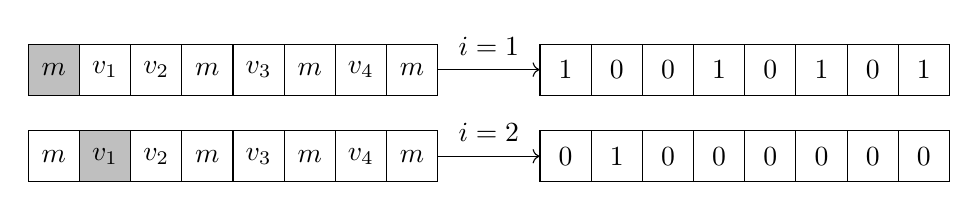
\begin{tikzpicture}
                    % 첫 번째 덩어리 (네 개의 정사각형)
                    \def\squareSize{0.65cm}
                    \node[draw, rectangle, minimum size=\squareSize, fill=gray!50] (a1) at (0, 0) {$m$};
                    \node[draw, rectangle, minimum size=\squareSize] (a2) at (\squareSize, 0) {$v_1$};
                    \node[draw, rectangle, minimum size=\squareSize] (a3) at (2*\squareSize, 0) {$v_2$};
                    \node[draw, rectangle, minimum size=\squareSize] (a4) at (3*\squareSize, 0) {$m$};
                    \node[draw, rectangle, minimum size=\squareSize] (a3) at (4*\squareSize, 0) {$v_3$};
                    \node[draw, rectangle, minimum size=\squareSize] (a4) at (5*\squareSize, 0) {$m$};   
                    \node[draw, rectangle, minimum size=\squareSize] (a3) at (6*\squareSize, 0) {$v_4$};
                    \node[draw, rectangle, minimum size=\squareSize] (aw) at (7*\squareSize, 0) {$m$};
                    
                    \node[draw, rectangle, minimum size=\squareSize] (be) at (10*\squareSize, 0) {$1$};
                    \node[draw, rectangle, minimum size=\squareSize] (b2) at (11*\squareSize, 0) {$0$};
                    \node[draw, rectangle, minimum size=\squareSize] (b3) at (12*\squareSize, 0) {$0$};
                    \node[draw, rectangle, minimum size=\squareSize] (b4) at (13*\squareSize, 0) {$1$};
                    \node[draw, rectangle, minimum size=\squareSize] (b5) at (14*\squareSize, 0) {$0$};
                    \node[draw, rectangle, minimum size=\squareSize] (b6) at (15*\squareSize, 0) {$1$};
                    \node[draw, rectangle, minimum size=\squareSize] (b7) at (16*\squareSize, 0) {$0$};
                    \node[draw, rectangle, minimum size=\squareSize] (b8) at (17*\squareSize, 0) {$1$};
                
                    \draw[->] (aw.east) -- (be.west);

                    \node[draw, rectangle, minimum size=\squareSize] (a1) at (0*\squareSize, -1.1) {$m$};
                    \node[draw, rectangle, minimum size=\squareSize, fill=gray!50] (a2) at (1*\squareSize, -1.1) {${v_1}$};
                    \node[draw, rectangle, minimum size=\squareSize] (a3) at (2*\squareSize, -1.1) {$v_2$};
                    \node[draw, rectangle, minimum size=\squareSize] (a4) at (3*\squareSize, -1.1) {$m$};
                    \node[draw, rectangle, minimum size=\squareSize] (a3) at (4*\squareSize, -1.1) {$v_3$};
                    \node[draw, rectangle, minimum size=\squareSize] (a4) at (5*\squareSize, -1.1) {$m$};    
                    \node[draw, rectangle, minimum size=\squareSize] (a3) at (6*\squareSize, -1.1) {$v_4$};
                    \node[draw, rectangle, minimum size=\squareSize] (cw) at (7*\squareSize, -1.1) {$m$};
                    
                    \node[draw, rectangle, minimum size=\squareSize] (ce) at (10*\squareSize, -1.1) {$0$};
                    \node[draw, rectangle, minimum size=\squareSize] (b2) at (11*\squareSize, -1.1) {$1$};
                    \node[draw, rectangle, minimum size=\squareSize] (b3) at (12*\squareSize, -1.1) {$0$};
                    \node[draw, rectangle, minimum size=\squareSize] (b4) at (13*\squareSize, -1.1) {$0$};
                    \node[draw, rectangle, minimum size=\squareSize] (b5) at (14*\squareSize, -1.1) {$0$};
                    \node[draw, rectangle, minimum size=\squareSize] (b6) at (15*\squareSize, -1.1) {$0$};
                    \node[draw, rectangle, minimum size=\squareSize] (b7) at (16*\squareSize, -1.1) {$0$};
                    \node[draw, rectangle, minimum size=\squareSize] (b8) at (17*\squareSize, -1.1) {$0$};
                
                    \draw[->] (cw.east) -- (ce.west);
                    
                    \node at (8.5*\squareSize, -0.8){$i=2$};
                    \node at (8.5*\squareSize, 0.3){$i=1$};
                \end{tikzpicture}
                \caption{Finding Common Values among $n$ Slots.} \label{fig: recover S}
            \end{figure}

    We first define two functions $\textsf{Duplicate}_i$ and $\textsf{Compare}$ as follows:
        \begin{itemize}
            \item $\textsf{Duplicate}_i: \bb Z_t^n \to \bb Z_t^n$ is a function that maps $(x_1, \dots, x_i, \dots, x_n) \mapsto (x_i, \dots, x_i)$
            \item $\textsf{Compare}(x,y):\bb Z_t^2\to \bb Z_t$ is $1$ if $x=y$ and $0$ if $x\neq y$.
        \end{itemize}
    We note that $\eval_{\textsf{Compare}}$ in BFV can be computed by Fermat's little theorem when its plaintext modulus $t$ is a prime, with $\lceil \log t \rceil$ homomorphic multiplications. But if $t=p^r$ for an integer $r>1$, we need a little modification.

    \begin{lemma}
        $\mathsf{Eval}_{\mathsf{Compare}}$ can be executed within $O(\log t)$ homomorphic multiplications in $\emph{BFV}$, both for $t=p$ and $t=p^r$ where $r>1$.
    \end{lemma}
    \begin{proof}
        Consider $e(x)=1-x^{\phi(t)}$ where $\phi$ is the Euler's totient function so that $e(x-y)=0$ if $x-y\in \bb Z_t^\times$, and otherwise $e(x-y)=1$. 
        If $t=p$, $e(x-y)$ is the desired $\mathsf{Compare}(x,y)$ function.
        Now suppose that $t=p^r$ and define a polynomial $\alpha$ as follows:
        \[
            \alpha(x):=e(x) \cdot \prod_{u\in \bb Z_t^\times\setminus \{1\}}(x+1-u).
        \] 
        Note that $\displaystyle\prod_{u\in \bb Z_t^\times\setminus \{1\}}(x+1-u)=\frac{(x+1)^{\phi(t)}-1}{(x+1)-1}=\sum_{i=0}^{\phi(t)-1}(x+1)^i,$ thus $\alpha$ can be evaluated within $O(\log t)$ homomorphic multiplications. Now we have three possible cases:

        \begin{enumerate}
            \item  If $x=0$, then $\alpha(0)=e(0)\cdot \phi(t)=\phi(t)$. 
            \item  If $x\in \bb Z_t^\times$, then $e(x)=0$ thus $\alpha(x)=0$.
            \item  If $x$ is a nonzero and non-unit, then $x+1\in \bb Z_t^\times\setminus\{1\}$. Thus 
                \begin{align*}
                   \alpha(x)&=e(x)\left(\prod_{u\in \bb Z_t^\times\setminus \{1\}}(x+1-u)\right)\\
                           &=e(x)\cdot 0=0.
                \end{align*}
        \end{enumerate}
        
        Therefore for $x,y\in \bb Z_t$, interpolating $\alpha(x-y)$ as $\phi(t)\mapsto 1$ and $0\to 0$ would give the desired $\textsf{Compare}(x,y)$ function.      
    \end{proof}

    Now we introduce Algorithm \ref{alg: common value position} to construct the desired circuit and describe its properties.
    
        \begin{algorithm}
            \caption{Finding Common Value Slots}
            \label{alg: common value position}
            \begin{algorithmic}[1]
                \Procedure{$\mathsf{CVS}$}{$\ct,i$}
                    \State $\ct'\gets\mathsf{\eval_{Duplicate}}_i(\ct)$ \Comment{$\ct'=\enc((x_i,\dots,x_i))$}
                    \State $\ct_{\textsf{CVS},i}\gets\eval_\mathsf{Compare}(\ct',\ct)$
                    \State \textbf{return} $\ct_{\mathsf{CVS},i}$
                \EndProcedure
            \end{algorithmic}
        \end{algorithm}
        \begin{lemma}
            For $i\overset{\$}{\gets}\{1,\dots,n\}$, {$\mathsf{CVS}(\mathsf{\ct},i)$} in the algorithm \ref{alg: common value position} outputs $\mathsf{Enc}(J_S)$ with probability of $|S|/n=1/2$ in $O(\log t)$ homomorphic multiplications and rotations.
        \end{lemma}
        \begin{proof}  
            Let $\ct$ be an encryption of a vector that has $m$ in computational slots $S^c$.
            If $i\in S^c$, then $\ct'\gets\eval_{\mathsf {Duplicate}_i}(\ct)$ is an encryption of $(m,\dots,m)$. Consequently, $\mathsf{Eval_{Compare}}(\ct',\ct)$ returns $\enc(J_S)$.
 
            $\eval_{\textsf{Duplicate}_i}$ requires one masking by the $i$-th elementary vector and a partial rotation sum within each message slot of length $n$ that takes $\lceil \log n \rceil$ homomorphic rotation. 
            Also we showed that \eval$_{\textsf{Compare}}$ needs $O(\log t)$ homomorphic multiplications. 
            Since $n\le \phi(t)$, the total complexity is $O(\log t)$ homomorphic multiplications/rotations.
        \end{proof}
        
    Now we show how to increase the success probability of the attack by repeating Algorithm \ref{alg: common value position} for different $i$'s.
    For any fixed $i$, if we sum up the values in the $n$ slots of $\ct_{\textsf{cvs},i}$, it outputs $|S|$ or $1$ depending on whether $i\in S$ or not. i.e. the server can {\em homomorphically distinguish} whether $i\in S$ or not.
    Using this principle, by repeating the algorithm \ref{alg: common value position}, the adversary can construct a cheating circuit that deterministically outputs $\enc(J_S)$. See Algorithm \ref{alg: deterministic attack on rep}.
    
    To design such circuit, first we define three functions $\textsf{RotSum},\textsf{Interpolate}$ and $\textsf{Normalize}_{k}$ as follows: 
        \begin{align*}
            \textsf{RotSum}&:\;(x_1,\dots,x_n) \mapsto \left(\sum_{i=1}^n x_i,\dots, \sum_{i=1}^n x_i\right)\\
            \textsf{Interpolate}&:\begin{cases}
            1\mapsto 0\\ n/2\mapsto 1\\ \text{otherwise anywhere.}\\    
            \end{cases}
            \textsf{Normalize}_k: \begin{cases}
                0\mapsto 0\\ 1,\dots,k \mapsto 1, \\ \text{otherwise anywhere}\\
            \end{cases}
        \end{align*}
    Note that $\eval_{\textsf{RotSum}}$ can be evaluated within $\lceil \log n \rceil$ homomorphic rotations, and $\eval_\textsf{Interpolate}, \eval_{\textsf{Normalize}_k}$ can be evaluated within $O(1)$ and $O(\log k)$ homomorphic multiplication respectively. 
    
        \begin{algorithm}
            \caption{Deterministic Recovery of Encryption of $S$}
            \label{alg: deterministic attack on rep}
            \begin{algorithmic}[1]
                \Procedure{$\mathsf{is\_in\_set}_S$}{$\ct,i$}
                    \State $\ct_{\textsf{cvs},i}\gets \textsf{CVS}(\ct,i)$
                    \State $\ct_{\textsf{rs}}\gets\textsf{RotSum}(\ct_{\textsf{cvs},i})$ \Comment{$\ct_{\textsf{rs}}=\enc(1,\dots,1)$ or $\enc(n/2,\dots,n/2)$}
                    \State $\ct_{\textsf{bool},i}\gets \eval_{\mathsf{Interpolate}}(\ct_{\textsf{rs}})$
                    \State \textbf{return} $\ct_{\textsf{bool},i}$ \Comment{$\ct_{\textsf{bool},i}=\enc(0,\dots,0)$ or $\enc(1,\dots,1)$}
                \EndProcedure
                    \State
                \Procedure{$\mathsf{Recover}_S$}{$\ct$}
                    \State $\ct_{\textsf{cvs},i}\gets \textsf{CVS}(\ct,i)$
                    \State $\ct_{\textsf{bool},i}\gets \textsf{is\_in\_set}_S(\ct,i)$
                    \State $\ct_S'\gets \sum_{i=1}^{n/2+1} \sf{Mult}(\ct_{\textsf{bool},i}, \ct_{\textsf{cvs},i})$
                    \State $\ct_S\gets \eval_{\textsf{Normalize}_{r}}(\ct_S')$
                    \State \textbf{return} $\ct_S$
                \EndProcedure
            \end{algorithmic}
        \end{algorithm}
        \begin{theorem} \label{thm: attack on rep}
            If the rotation key with index 1 is given, $\mathsf{Recover}_S(\mathsf{ct})$ in Algorithm \ref{alg: deterministic attack on rep} can be evaluated within a computational cost of $O(n \log t)$, deterministically outputting $\enc(J_S)$. 
        \end{theorem}
        \begin{proof}
            Since the slots in $\ct_{\textsf{cvs},i}$ contain $n/2$ ones if $i\in S^c$, and a single one if $i\in S$, applying $\eval_{\textsf{RotSum}}$ yields either 
            $\enc\left(\frac{n}{2},\dots,\frac{n}{2}\right)$ or $\enc(1,\dots,1).$
            Consequently, by interpolation, the output $\ct_{\text{bool},i}$ is a vector of Boolean values, either $(1,\dots,1)$ or $(0,\dots,0)$. Thus, for $i=1,\dots,n/2+1$, the sum of the $\ct_{\textsf{cvs},i}$ after homomorphic multiplication with $\ct_{\text{bool},i}$ decrypts to the same value as 
            $|S^c\cap\{1,\dots,n/2+1\}|\cdot \enc(J_S).$
            Since $S\subset\{1,\dots,n\}$ is a random subset of size $n/2$, $|S^c\cap\{1,\dots,n/2+1\}|$ is nonzero.
            Thus, after evaluating $\textsf{Normalize}_{1+n/2}$, we obtain $\enc(J_S)$ with these probabilities.

            Furthermore, the procedure $\mathsf{Recover}_S(\ct)$ calls $\textsf{CVS}_i$ for $i=1,\dots,n/2+1$, which incurs a cost of $O(n\log t)$ homomorphic operations. The cost of the remaining operations does not exceed $O(n\log t)$.
        \end{proof}
        \begin{corollary}\label{Cor: Rep}
            $\sf \REP$ is not secure against the presence of $\cc A_c^{\rtk_1}$.
        \end{corollary}
        \begin{corollary}
            If BFV bootstrapping needs $\rtk_1$, $\sf \REP$ is not bootstrappable or insecure against $\cc A_c$.
        \end{corollary}

    \subsection{Attack on Replication Encoding with Multiple Secret Keys}\label{subsec: diff keys}

        \subsubsection{Patch on \REP{} using Multiple Secret Keys.}
        We introduce $\REP^{\sf MSK}$, a countermeasure to the previous deterministic attack. The previous attack evaluates homomorphic rotations to compare values in different slots and recover $\enc(J_S)$. 
        Notably, a rotation key with index 1 is essential for executing this attack. Meanwhile, in $\REP$, a single value $m$ is encoded into $n$ slots. Therefore, to perform operations on two values $m_1$ and $m_2$ encoded via $\REP$, only rotation keys whose index is a multiple of $n$ will be required. Nevertheless, we note that a rotation key with index 1 remains essential for the bootstrapping of homomorphic encryption. Thus, the idea of preventing the above attack by not providing a rotation key with index 1 is not adequate. 
        
        Instead of restricting the rotation key with index 1, we consider the following possibility: Replicate the messages into $n$ different ciphertexts encrypted with \emph{different keys}. This would prevent interoperability between ciphertexts, making it difficult for the adversary to homomorphically determine in which slots the messages belong to.
        First, prepare a random subset $S \subset \{1, \dots, n\}$ with $|S| = n/2$, a message $m \in \bb Z_t$, and verification values $v_i \gets \bb Z_t$ for $i \in S$. 
        Next, generate $n$ different keys $\{\pk_i, \sk_i, \mathsf{evk}_i\}$ for $i \in \{1, \dots, n\}$.
        Now, instead of encrypting messages as a vector, we encrypt them elementwisely, i.e. $\ct_i = \enc_{\pk_i}(m)$ for $i \in S$ and $\ct_i = \enc_{\pk_i}(v_i)$ for $i \notin S$.
        Then, the server can compute those ciphertexts with different $\evk_i$'s.
        This patch achieves the same effect as the original \REP{} while preventing the previous attack in Algorithm~\ref{alg: deterministic attack on rep} by restricting the homomorphic comparison, while still providing the bootstrapping functionality. 
        
            \begin{figure}
                \centering
                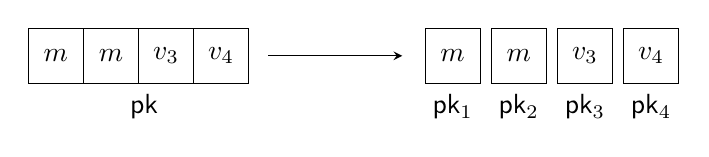
\begin{tikzpicture}
                    \def\squareSize{0.7cm}
                    \def\adjust{0cm}
                    \node[draw, rectangle, minimum size=\squareSize] (a1) at (10.2*\squareSize-\adjust, 2) {$m$};
                    \node at (10.2*\squareSize-\adjust, 1.35) {$\pk_1$};
                    \node[draw, rectangle, minimum size=\squareSize] (a2) at (11.4*\squareSize-\adjust, 2) {$m$};
                    \node at (11.4*\squareSize-\adjust, 1.35) {$\pk_2$};
                    \node[draw, rectangle, minimum size=\squareSize] (a3) at (12.6*\squareSize-\adjust, 2) {$v_3$};
                    \node at (12.6*\squareSize-\adjust, 1.35) {$\pk_3$};
                    \node[draw, rectangle, minimum size=\squareSize] (a4) at (13.8*\squareSize-\adjust, 2) {$v_4$}; 
                    \node at (13.8*\squareSize-\adjust, 1.35) {$\pk_4$};
                    
                    \node[draw, rectangle, minimum size=\squareSize] (a3) at (3*\squareSize, 2) {$m$};
                    \node[draw, rectangle, minimum size=\squareSize] (a4) at (4*\squareSize, 2) {$m$}; 
                    \node[draw, rectangle, minimum size=\squareSize] (a3) at (5*\squareSize, 2) {$v_3$};   
                    \node[draw, rectangle, minimum size=\squareSize] (aw) at (6*\squareSize, 2) {$v_4$};  
        
                    \node at (4.6*\squareSize-\adjust, 1.35) {$\pk$};
                    
                    \draw[-stealth] (4.8, 2) -- (6.5, 2);
                \end{tikzpicture}
                \caption{Encryption with different keys. \label{fig: enc with diff keys}}
            \end{figure}
        
        However, we can also attack $\REP^{\sf MSK}$ similarly to our attack on vADDG, namely, by implementing a pseudorandom characteristic function. It is possible since the evaluation does not rely on homomorphic rotation or comparison but only on slot-wise operations. 
        We analyze how this attack applies to this variant. Moreover, in vADDG, it was able to patch the attack by increasing the number of verification values by adjusting some parameters. We intend to investigate whether the same approach can be applied to patch $\REP^{\sf MSK}$ or not.

        \subsubsection{Attack on $\REP^{\sf MSK}$.} \label{subsec:3.3 Extended Attack}
        First, let the adversary fix a random subset $A\subset \bb Z_t$ where the message $m$ is expected to belong. 
        Next, evaluate $\chi_A$ homomorphically on a ciphertext.
        After evaluating $\chi_A$, it becomes possible to forge the values that exactly belong to $A$.
        If $\{m,v_i:i\in S\}\cap A = \{m\}$, then ${\sf CMult}$ between $\ct_S:=\eval_{\chi_A}(\ct)$ and the encoding of the vector $(\overbrace{1,\dots,1}^{n},\overbrace{0,\dots,0}^{N-n})$ is an encryption of a vector $(J_{S^c}\,\Vert\,\overbrace{0\dots0}^{N-n})$.
        
            \begin{algorithm}
                    \caption{Extended Attack on \REP}
                    \label{alg: probabilistic attack on rep}
                    \begin{algorithmic}[1]
                        \Procedure{$\mathsf{Extended\_Attack}$}{$\ct, A$}
                            \State $\ct_{\textsf{bool}}\gets \textsf{Eval}_{\chi_A}(\ct)$
                            \State $\mathsf{pt}_{\textsf{Masking}}\gets (\overbrace{1,\dots,1}^{n},\overbrace{0,\dots,0}^{N-n})$
                            \State $\ct_{S}\gets\textsf{CMult}(\ct_{\sf bool},\mathsf{pt}_{\sf Masking})$ 
                            \State \textbf{return} $\ct_{S}$
                        \EndProcedure
                    \end{algorithmic}
            \end{algorithm}
            
        Let us calculate the attack success probability with respect to the size of $A$. 
        Since $A$ is chosen randomly, the success probability of the attack depends only on the size of $A$. 
        Let $p=|A|/{t}$ be the probability of each element $m$ or $v_i$ belonging to the set $A$. 
        Set $q := 1 - p$ and $\mu:=\left|\{m,v_i:i\in S\}\right|=1+\frac{n}{2}$. 

            \begin{theorem}\label{thm2: univ}
                Let $A$ be a randomly chosen subset of $\bb Z_t$ with size $|A|=p\cdot t$. For $\ct_S\gets\mathsf{Extended\_Attack}(\ct,A)$ in the Algorithm \ref{alg: probabilistic attack on rep}, the probability $$\Pr\left[\mathsf{Dec}(\ct_S)=(J_{S^c}\Vert\overbrace{0\dots0}^{N-n})\right]=:Q(p)$$ is maximized when $p=\mu^{-1}=\frac{1}{1+(n/2)}$. Also $Q(p)>e^{-1}p$ when restricted to $p=\mu^{-1}.$
            \end{theorem}
            \begin{proof}
                Let's define $\cc V:=\{m,v_i:i\in S\}$. Then, there are three possible cases: 
                    \begin{itemize} 
                        \item Case (1): $\cc V\cap A=\emptyset$. The probability is $q^{\mu}$.
                        \item Case (2): $\{v_i:i\in S\}\cap A\neq\emptyset$. The probability is $1-q^{\mu-1}$. 
                        \item Case (3): $\cc V \cap A=\{m\}$. The probability is $q^{\mu-1}-q^{\mu}$. 
                    \end{itemize}
                Nothing happens in the case (1), and the adversary is caught in the case (2). The case (3) is the case of a successful attack. 
                Now represent the probability of case (3) $Q(p)$ in terms of $p$. 
                \begin{align*}
                    Q(p)=&q^{\mu-1}-q^\mu \\
                    =&(1-p)^{\mu-1}-(1-p)^{\mu}.
                \end{align*} 
            By simple calculus, one can verify that $\frac{dQ}{dp}(\mu^{-1})=0$ and $Q(p)$ is maximized when $p=\mu^{-1}$: $$Q(\mu^{-1})=(1-\mu^{-1})^{\mu-1}-(1-\mu^{-1})^{\mu}=(1-p)^{(1/p)-1}-(1-p)^{(1/p)}.$$
            Now let $R(p):=(1-p)^{(1/p)-1}-(1-p)^{(1/p)}$. Then, $\lim_{p\to 0+}\frac{dR}{dp}(p)=e^{-1}$ and $\frac{d^2R}{dp^2}>0$. Thus 
            $R(p)>e^{-1}p$.
            % See Fig. \ref{q} for their graphs.
            \end{proof}
            % \begin{figure}
            %     \centering
            %         \begin{tikzpicture}
            %             \begin{axis}
            %             [
            %                 axis lines=middle,
            %                 xmin=0, xmax=1.1,
            %                 ymin=0, ymax=1.1,
            %                 xlabel={$p$},
            %                 ylabel={},
            %                 domain=0:1,
            %                 samples=400,
            %                 width=5cm,
            %                 height=4cm,
            %                 xtick={0,1},
            %                 ytick={0,1},
            %                 enlargelimits=true
            %             ]
            %             \addplot[blue, thick] {x/e};
            %             \addplot[red, thick] {(1-x)^((1-x)/x) - (1-x)^(1/x)};
            %             \end{axis}
            %         \end{tikzpicture}
            %     \caption{The graphs of $R(p)$ (red) and $e^{-1}p$ (blue).} \label{q}
            % \end{figure}
        Therefore, for any given parameter $\mu=1+(n/2)$, if the adversary randomly chooses a subset $A$ so that $p=|A|/t$ is approximately $\mu^{-1}$, and homomorphically evaluates $\chi_A$, then the adversary's advantage is maximized with a probability at least $({e \mu})^{-1}$.
        
        Thus, unlike in the vADDG attack where a countermeasure was possible by adjusting parameters, in this variant of \REP{} a forgery attack can be mounted with non-negligible probability. However, under the assumption of a covert adversary model, such an attack is not feasible. 

        % Meanwhile, considering the covert adversary scenario, let us derive the probability of being caught when a forgery occurs. This probability is given by \(\frac{1-q^{\mu-1}}{1-q^\mu}\geq\frac{\mu-1}{\mu},\)
        % thus the adversary is caught with a probability of at least \(\frac{\mu-1}{\mu}\).
        % Thus the covert adversary cannot execute this attack.

        \paragraph{Pseudo-Random Characteristic Function on BFV.}
        The attack cost in Theorem~\ref{thm2: univ} is determined by the evaluation cost of the characteristic function. In the attack on VOPRF, the evaluation was straightforward since extracting encrypted bits from the TFHE ciphertext string was easy. However, in BFV, homomorphically evaluating \(\chi_A\) for any randomly given subset \(A\) with the full support \(\mathbb{Z}_t\) generally requires \(O(\sqrt{t})\) homomorphic operations, which results in an exponential cost with respect to \(\log t\). Therefore, it is necessary to devise an efficient method for evaluating a pseudorandom characteristic function over \(\mathbb{Z}_t\).
        
       
        Before constructing a pseudo-random characteristic function, we note that the pseudorandom characteristic function used in this attack does not need to be cryptographically secure; rather, it is sufficient for it to be a function that heuristically produces an unbiased uniform distribution.
        
        To construct an efficient pseudo-random characteristic function, we assume the pseudo-randomness of the distribution of the roots of unity in $\bb Z_t$:
        For an integer $t$ and $d \mid \phi(t)$, let $U_{t,d}:=\{x\in \bb Z_t^\times:x^{\phi(t)/d}=1\} \subset \bb Z_t^\times$. We assume that this subset $U_{t,d}$ of size $\phi(t)/d$ is an unbiased sample from a uniform distribution of $(\phi(t)/d)$-combinations from $\bb Z_t^\times$. Specifically, for a large odd prime $p$, $U_{p,2}$ is the set of quadratic residues modulo $p$, whose pseudo-randomness is utilized to construct the Legendre PRF~\cite{LPRF}. Although the specific assumptions and parameters in here are different from those of Legendre PRF, we again note that it is sufficient for it to be a function that heuristically produces an unbiased uniform sampling.
        
        Now we state the property of the characteristic function $\chi_{U_{t,d}}: \bb Z_t\to\{0,1\}$ for $t=p^r$.
        Before proof, note that $a\in \bb Z_{p^r}$ is a zero divisor if and only if $a \equiv 0\pmod p$. 
        
        \begin{lemma}\label{bfvprf} For $t=p^r$ and $d \mid (p-1)$, we have
            $$d\cdot \chi_{U_{t,d}}(x)=x^{\phi(t)}\cdot\sum_{i=0}^{d-1} \left(x^{\phi(t)/d}\right)^i.$$
        \end{lemma}
        \begin{proof}
        \begin{enumerate}
            \item First, suppose that $x$ is a non-unit. Then the left-hand side $(\sf LHS)$ is $0$. Also as $x$ is a multiple of $p$, the right-hand side $(\sf RHS)$ is also $0$ since it would be multiple of $p^{\phi(t)}\equiv0 \pmod{p^r}$. 
            \item Next, suppose that $x\in U_{t,d}$. Since $x$ is a unit, $x^{\phi(t)}=1$. Also $x^{\phi(t)/d}=1$ by definition. Thus both $\sf LHS$ and $\sf RHS$ are equal to $d$.
            \item Lastly, suppose that $x\in \bb Z_t^\times\setminus U_{t,d}$. Since $x$ is a unit, $x^{\phi(t)}=1$. Also $x^{\phi(t)/d}\neq 1$ by definition, while $(x^{\phi(t)/d})^d-1=(x^{\phi(t)/d}-1)\left(\sum_{i=0}^{d-1} \left(x^{\phi(t)/d}\right)^i\right)=0$.
            Thus, $\sum_{i=0}^{d-1} \left(x^{\phi(t)/d}\right)^i=0$ or both $x^{\phi(t)/d}-1, \sum_{i=0}^{d-1} \left(x^{\phi(t)/d}\right)^i$ are zero-divisors. We exclude the second case to conclude that $\sf RHS=0$: For $y=x^{\phi(t)/d}$, if $y-1$ is a zero divisor, then $y=pm+1$ for some integer $m$, consequently $\sum_{i=0}^{d-1} \left(x^{\phi(t)/d}\right)^i\equiv d\not\equiv0 \pmod p.$ Thus it is not a zero divisor, a contradiction. 
        \end{enumerate} 
        \end{proof}
        Note that if $t$ is a prime, then the $x^{\phi(t)}$ term is not needed. Also, note that this function can be homomorphically evaluated using $O(\log t)$ homomorphic multiplications with a multiplication depth of $\lceil\log\phi(t)\rceil$.
        
        By homomorphically evaluating $\chi_{U_{t,d}}(x+a)$ for a random integer $a$ and appropriate $d\mid (p-1)$ with asymptotic size $d\approx\mu$, the adversary can construct a characteristic function $\chi_A$ with an asymptotic size of $|A|=\phi(t)/d \approx \lfloor t / \mu \rceil$ to achieve the maximal attack probability in the Theorem \ref{thm2: univ}. If necessary, the adversary may evaluate several characteristic functions to construct another size of characteristic function.\footnote{For example, one may utilize the formula $\chi_A(x) \cdot \chi_B(x) = \chi_{A \cap B}(x).$}

        \begin{corollary}
            $\sf REP^{\sf MSK}$ is not secure against the presence of $\cc A_m.$
        \end{corollary} 
        Whether there exists a method to successfully execute a forgery attack with overwhelming probability remains an open question.
         
%%%%%%%%%%%%%%%%%%%%%%%%%%%%%%
%       Section 5
%%%%%%%%%%%%%%%%%%%%%%%%%%%%%%

\section{Cryptanalysis on Polynomial Encoding} \label{sec:PE}

    \subsection{Polynomial Encoding}
    There is another suggested scheme for verifiable HE in \cite{VE}, the Polynomial Encoding (\PE).
    Its plaintext space and ciphertext space are BFV plaintext/ciphertext space but with a new indeterminate $Y$. 
    More precisely, its encryption is 
        \[
            \bb{Z}^N_t[Y] \overset{\enc_\PE}{\longrightarrow} \mathcal{R}^2_q[Y],
        \]
    where the $\enc_\PE$ is the coefficient-wise BFV encryption.
    To avoid confusion, we represent the elements of $\mathcal{R}^2_q[Y]$ using capitalized sans-serif font: $\mathsf{F}(Y) = \ct_0 + \ct_1 Y + \dots + \ct_d Y^d$. 
    We refer to $\mathsf{F}(Y)$ as a ciphertext polynomial and each of its coefficients as a ciphertext.

    Encryption in \PE{} proceeds as follows: 
    For the number of slots $N$, a random verification value $\mathbf{v}=(v_1,\dots, v_N)\in \bb Z_t^N$ and a secret value $\alpha \in \mathbb{Z}_t^\times$ are chosen. 
    Then, the message $\mathbf{m}=(m_1,\dots,m_N)\in \bb Z_t^N$ and the verification value $\mathbf{v}$ are interpolated at $Y = 0$ and $Y = \alpha$, respectively. 
    After that, each message is encrypted coefficient-wisely:
    
        \begin{center}
            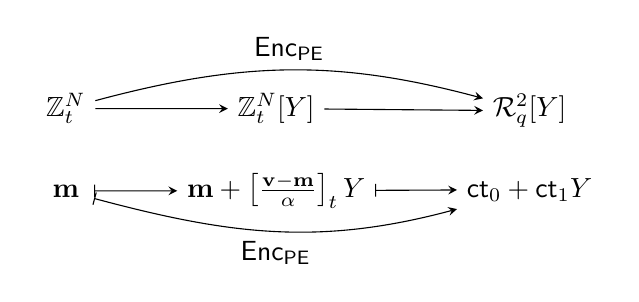
\begin{tikzpicture}
                  \matrix (m) [matrix of math nodes,row sep=1em,column sep=3em,minimum width=2em]
                        {
                            \bb Z^N_t & \bb Z^N_t[Y] & \cc R^2_q[Y]\\
                            \mathbf{m}& \mathbf{m}+\left[\frac{\mathbf{v-m}}{\alpha}\right]_tY&\ct_0+\ct_1Y\\
                        };
                  \path[]
                        (m-1-1) edge [-stealth] (m-1-2)
                        (m-1-2) edge [-stealth] (m-1-3)
                        (m-1-1) edge [-stealth, out=15, in=165] node[above]{$\enc_\PE$} (m-1-3)
                        
                        (m-2-1) edge [|-stealth, out=-15, in=195] node[below] {$\enc_\PE$}(m-2-3)
                        (m-2-2) edge [|-stealth] (m-2-3)
                        (m-2-1) edge [|-stealth] (m-2-2);
            \end{tikzpicture}
        \end{center}
        
    The server coefficient-wisely performs homomorphic operations like addition, constant multiplication, rotation, and even bootstrapping, except for multiplication. 
    The multiplication is evaluated as a polynomial in $Y$:
    For example, the multiplication between two ciphertext polynomials $\ct_0+\ct_1Y$ and $\ct_2+\ct_3Y$ is 
        \[
            \mathsf{Mult}(\ct_0,\ct_2)+\mathsf{Mult}(\ct_1,\ct_2)Y+\mathsf{Mult}(\ct_0,\ct_3)Y+\mathsf{Mult}(\ct_1,\ct_3)Y^2.
        \]
    If the server has performed the operations correctly, the result $\mathsf F(Y)\in \cc R^2_q[Y]$ satisfies $\dec(\mathsf F(0)) = f(\mathbf{m})$ and $\dec(\mathsf F(\alpha)) = f(\mathbf{v})$. 
    In the verification step, the client checks whether $\dec(\mathsf F(\alpha))=f(\mathbf{v})$ and if it is correct, accepts $\dec(\mathsf F(0))$ as $f(\mathbf{m})$.
    
        \subsubsection{Re-Quadratization Protocol.} 
        As the computation progresses, the degree of $Y$ increases exponentially, leading to significant computational overhead. To mitigate this, \cite{VE} proposed a client-assisted computing protocol called the Re-Quadratization (\REQ) protocol.
        This protocol makes a quartic polynomial $\mathsf{Q}_4(Y)\in \cc R^2_q[Y]$ into a quadratic polynomial $\mathsf{Q}_2(Y)\in \cc R^2_q[Y]$ while ensuring that $\dec(\mathsf{Q}_4(0))=\dec(\mathsf{Q}_2(0))$.
    
        However, if $\dec(\mathsf{Q}_4(\alpha)) = \mathbf{a}$, 
        then $\dec(\mathsf{Q}_2(\alpha)) = \mathbf{a} + \mathbf{r}$ 
        for some uniform random blinding vector $\mathbf{r} \in \mathbb{Z}_t^N$.
        Because of this random blinding vector $\mathbf{r}$, the client must compute and handle the deviations of the circuit introduced by $\mathbf{r}$.
        For instance, when performing squaring 
        \(
        (\mathbf{a} + \mathbf{r})^2 
        = \mathbf{a}^2 + 2\mathbf{a}\mathbf{r} + \mathbf{r}^2,
        \)
        the user must compute the deviation $2\mathbf{a}\mathbf{r} + \mathbf{r}^2$ and subtract it to recover $\mathbf{a}^2$ in the \REQ{} protocol. This self-correctness property through client-side computation forces the client to perform as much computation as if the client itself were running the delegated computation in plaintext, negating much of the intended benefit of HE.
%        \footnote{In the scenario where \REQ{} does not introduce random blinding, another interesting cryptanalysis exists: The adversary can learn the encryption of $\alpha$. See Appendix \ref{Appendix A} for details.}
        
        Despite this drawback, the \REQ{} protocol reduces the computational overhead of homomorphic computation via \PE.
        If the server multiplies two quadratic polynomials $\mathsf{Q_2}(Y)$, $\mathsf{Q}'_2(Y)$ and gets a quartic polynomial $\mathsf{Q_4}(Y)$, then the server can use \REQ{} to reduce $\mathsf{Q}_4(Y)$ back to a quadratic polynomial $\mathsf{Q}''_2(Y)$. Therefore the server can evaluate a deep circuit avoiding an exponential overhead.
        See V.D. and Appendix E in \cite{VE} for details.
        Here, we only use \REQ{} protocol as an oracle for avoiding overhead in deep circuit evaluation.
      
    \subsection{Attack on Polynomial Encoding}
    Now we present the attack on the Polynomial Encoding. We assume that the \REQ{} protocol serves as a subroutine in the computation. 
    
    Let $f(x_1,\dots, x_k)$ be an honest polynomial circuit that operates on the ciphertext polynomial space $\mathcal{R}^2_q[Y]$.
    Given $k$ inputs $\mathsf{L}_i(Y) = \ct^{(0)}_i + \ct^{(1)}_i Y$ for $i=1,\dots, k$, the polynomial circuit $f$ processes these inputs and produces the output
    \(
        f(\mathsf{L}_1(Y), \dots, \mathsf{L}_k(Y)) = \mathsf{F}(Y) \in \mathcal{R}^2_q[Y].
    \)
    When evaluated at $Y = \alpha$, we obtain
    \[
        \mathsf{F}(\alpha) = \eval_f(\ct_1^{(0)}+\alpha\cdot\ct_1^{(1)}, \dots, \ct_k^{(0)}+\alpha\cdot\ct_k^{(1)}) = \enc(f(v_1, \dots, v_k)).
    \]
    Now let $g$ be any malicious polynomial circuit that outputs $\mathsf{G}(Y)$. Similarly, when evaluated at $Y=0$, it has
    \[
        \mathsf{G}(0) = \eval_g(\ct_0^{(0)}, \dots, \ct_k^{(0)}) = \enc(g(m_1, \dots, m_k)).
    \]
    Since only the result $\sf G(0)$ will be needed, the circuit $g$ does not need to act on the entire ciphertext polynomial; it only needs to operate on its constant term, namely $\ct_0^{(0)}, \dots, \ct_k^{(0)}$. Consequently, the evaluation of $g$ does not require \REQ{}.
    To forge the result, we introduce a trick: define $\mathsf{L}^\star(Y):= \enc(u_1,\dots,u_N) Y$ where all $u_i\in \bb Z_t^\times$. For the polynomial circuit $p(y) := y^{\phi(t)}$, evaluating $p$ at $\mathsf{L}^\star(Y)$ yields $\mathsf P(Y)$ which satisfies
    \[
        \mathsf{P}(0) = p(\mathsf{L}^\star(0)) = \enc(0,\dots,0), \quad \mathsf{P}(\alpha) = p(\mathsf{L}^\star(\alpha)) = \enc(1,\dots,1). 
    \]
    Thus, if we evaluate the following polynomial circuit
    \[
        h(y_1, \dots, y_k, \ell^\star) := g(\tilde y_1, \dots, \tilde y_k) + (f(y_1, \dots, y_k) - g(\tilde y_1, \dots, \tilde y_k)) p(\ell^\star)
    \]
    at $\left(y_1,\dots,y_k,\ell^\star\right)\gets\left(\mathsf{L_1}(Y),\dots,\mathsf L_{k}(Y),\mathsf{L}^\star(Y)\right)$ where $\tilde y_i=\mathsf{L}_i(0)$ for $y_i=\mathsf{L}_i(Y)$,
    the output $\mathsf{H}(Y)$ satisfies
    \[
        \dec(\mathsf{H}(0)) = \dec(\mathsf{G}(0)), \quad \dec(\mathsf{H}(\alpha)) = \dec(\mathsf{F}(\alpha))
    \]
    which successfully passes the verification and gives the forged results.

        \begin{algorithm}
            \caption{Attack against \PE}
            \label{alg: Attack against PE}
            \begin{algorithmic}[1]
                \Procedure{$\mathsf{PE\_Attack}$}{$\{\mathsf L_i(0)\}, \mathsf F(Y)$} \Comment{$\{\mathsf L_i(Y)\}_{1\leq i\leq k}$ are input points, \begin{flushright}
                    $\mathsf F(Y)$ is a honest result.
                \end{flushright}}
                    \State $\ct_{\sf forged}\gets \eval_g(\mathsf L_1(0),\dots, \mathsf L_k(0))$ \Comment{$g$ is any circuit different from $f$.}
                    \State $\mathsf L^\star(Y)\gets\enc(u_1,\dots,u_N)Y$ \Comment{Every $u_i$ is a unit.}
                    \State $\mathsf P(Y)\gets p({\sf L}^\star (Y))$ \Comment{$p(y)=y^{\phi(t)}$.}
                    \State $\mathsf H(Y)\gets \ct_{\sf forged}+(\mathsf{F}(Y)-\ct_{\sf forged})\cdot \mathsf{P}(Y)$
                    \State \textbf{return} $\mathsf H(Y)$
                \EndProcedure
            \end{algorithmic}
        \end{algorithm}
    
    Now we have the following theorem.
        \begin{theorem}
            If the adversary can access the $\REQ$ protocol, Algorithm \ref{alg: Attack against PE} can be executed within the cost of $O(\log t)$ with deterministic output ${\sf H}(Y)$.
        \end{theorem}
        \begin{proof}
            The correctness of the attack circuit is given above.
            Take $g$ to be a constant circuit different from $f$. Then the compuational cost is determined by evaluating $p(y)=y^{\phi(t)}$ at $y=\mathsf L^\star (Y)$, which requires $\lceil\log(\phi(t))\rceil$ multiplications in $\cc R^2_q[Y]$ and $\REQ$ protocol. Therefore the total computational complexity is $O(\log t)$.
        \end{proof}

        \begin{corollary}
            $\PE$ is not secure against the presence of $\cc A_c^{\cc O_{\sf ReQ}}.$
        \end{corollary}
        
%%%%%%%%%%%%%%%%%%%%%%%%%%%%%%
%       Section 6
%%%%%%%%%%%%%%%%%%%%%%%%%%%%%%

\section{Implementation}\label{sec: Implementation}

We implemented our attacks on the Oblivious Ride Hailing implementation in the \textsc{Veritas} library, which is based on the Lattigo BFV Implementation~\cite{Lattigo}. Specifically, we implemented the attack on $\REP$ (Algorithm~\ref{alg: deterministic attack on rep}) as well as the attack on $\REP^{\sf MSK}$ (Algorithm~\ref{alg: probabilistic attack on rep}). Since the Lattigo library currently does not support BFV bootstrapping, we modified the value of $t$ in the parameters provided by the example code in the \textsc{Veritas} library to ensure that the forgery circuit operates without bootstrapping. However, when bootstrapping is supported, the attack remains feasible regardless of the value of $t$
\footnote{For \PE, \(t\) must be of size roughly equal to the security parameter \(\lambda\), since the secret \(\alpha\) is chosen from \(\mathbb{Z}_t^\times\). With this parameter setting, the implementation of the attack is not feasible without bootstrapping. Thus we did not implement this attack on \PE.}.

As for vADDG, since the verifiable variant is not implemented, we did not implement the attack. However, since the attack circuit is very shallow and simple, and in particular very similar to the attack on $\REP^{\sf MSK}$, the feasibility of the attack on vADDG is straightforward even without a demonstration via implementation. 
 
\subsection{Attack Results}
The experiments were performed on an Intel(R) Xeon(R) Silver 4114 CPU at 2.20GHz running Linux in a single-threaded environment. The detailed parameters and the corresponding attack results are summarized in Tables~\ref{tab: Params},~\ref{tab:Cost},~\ref{tab:Prob}. The time cost only measured evaluation time. We note that the attack cost is the difference between the evaluation costs of the honest and cheating circuits, not determined by the ratio between them.
\begin{table}[htb!]
\centering
\begin{tabular}{|cc|c|c|c|c|}
\hline
\multicolumn{2}{|c|}{Parameters} & $\log N$ & $\log Q$ & $t$ & $n$ \\ \hline
\multicolumn{1}{|c|}{\makecell{\REP{} Attack}} & Exp1 &  {16} & {1440} &  {$2^{19}+2^{18}+1$} & 64\\ \hline 
\multicolumn{1}{|c|}{\multirow{2}{*}{\makecell{$\REP^{\sf MSK}$Attack}}} & Exp2 & \multirow{2}{*}{15} & \multirow{2}{*}{700} & \multirow{2}{*}{$2^{16}+1$} & 64 \\ \cline{2-2} \cline{6-6} 
\multicolumn{1}{|c|}{} & Exp3 &  &  &  & 32\\ \hline
\end{tabular}
\caption{Parameters Selection}
\label{tab: Params}
% \end{table}

% \begin{table}[htb!]
% \centering
\begin{tabular}{|cc|c|c|c|}
\hline
\multicolumn{2}{|c|}{\makecell{Evaluation Time\\(Sec/op)}} & \makecell{Honest Circuit\\Evaluation} & \makecell{Cheating Circuit\\Evaluation} & \makecell{Time Difference\\ (Attack Cost)} \\ \hline

\multicolumn{1}{|c|}{\makecell{\REP{} Attack}} & Exp1 & 2.47s & 1417.45s & 1414.08s \\ \hline

\multicolumn{1}{|c|}{\multirow{2}{*}{\makecell{$\REP^{\sf MSK}$Attack}}} & Exp2 & 0.31s &  5.94s & 5.63s  \\ \cline{2-5} 
\multicolumn{1}{|c|}{} & Exp3 & 0.31s & 5.41s & 5.10s \\ \hline
\end{tabular}
\caption{Circuit Evaluation Cost}
\label{tab:Cost}

% \end{table}

% \begin{table}[htb!]
% \centering
\begin{tabular}{|cc|c|c|c|}
\hline
\multicolumn{2}{|c|}{Probability} & \makecell{Theoretical Attack \\ Success Probability} & \makecell{Experimental Attack \\ Success Probability} & {\# of Iterations}\\ \hline

\multicolumn{1}{|c|}{\makecell{\REP{} Attack}} & Exp1 & 100\% & 100\% & 1 \\ \hline

\multicolumn{1}{|c|}{\multirow{2}{*}{\makecell{$\REP^{\sf MSK}$Attack}}} & Exp2 & 1.13\% & 0.80\% &  1000 \\ \cline{2-5} 
\multicolumn{1}{|c|}{} & Exp3 & 2.22\% & 3.60\% & 500 \\ \hline
\end{tabular}
\caption{Attack Success Probability}
\label{tab:Prob}
\end{table}

\subsubsection{Attack on \REP.}
In experiment 1, we implement the attack on $\REP$ described in \ref{alg: deterministic attack on rep}. We generated keys whose rotation indices are divisors of \( n \), assuming a scenario in the adversarial server needs to bootstrap with these rotation keys.
To optimize the attack circuit, we modified \(\eval_{\sf Interpolate}\) in Algorithm~\ref{alg: deterministic attack on rep} to perform \(\ct \mapsto \ct - \enc(1,\dots,1)\) and omitted \(\eval_{{\sf Normalize}_{r}}\). As a result, we obtain a constant multiple of \(J_{S^c}\). 

This attack circuit can be implemented without bootstrapping under the parameters \((\log N = 15, \log Q = 700)\). However, due to issues with the large multiplication depth of the circuit, the attack failed with approximately half probability due to the noise budget issue. Nevertheless, this failure is not due to a flaw in the attack itself but rather a limitation arising from the inability to perform bootstrapping. Since this attack assumes a scenario in which the adversarial server possesses \(\rtk_1\) for bootstrapping, it does not contradict the result of Corollary~\ref{Cor: Rep}.  
Instead, we implemented the attack using parameters \((\log N = 16, \log Q = 1440)\), which provide a larger noise budget.
Due to the large \(N\) and the replication number \(n\), evaluating the cheating circuit incurs a substantial computational cost. Nevertheless, the attack remains feasible within 30 minutes. Moreover, since Algorithm~\ref{alg: deterministic attack on rep} is inherently parallelizable, leveraging GPU optimization could potentially reduce the runtime to just a few seconds. This assumption is highly realistic, as adversaries in the context of VHE are generally considered to possess extremely high computational power.

\subsubsection{Attack on $\REP^{\sf MSK}.$}
In experiments 1 and 2, we implement the attack on $\REP^{\sf MSK}$ described in Algorithm \ref{alg: probabilistic attack on rep}. Since this attack naturally applies to $\REP$, without any modification to the $\REP$ scheme we implemented this attack: Specifically, we did not generate the $\rtk_1$. To optimize the attack circuit, we employed the following strategy: Since \(\phi(t)=2^{16}\), when constructing the characteristic function in Lemma~\ref{bfvprf}, we can choose \(d\) to be a power of 2. In Experiment 2, where \(n=64\), we set \(d=32 \cong \mu=33\) for the characteristic function. According to Theorem~\ref{thm2: univ}, the corresponding expected attack success probability is $(1-\frac{2^{11}}{2^{16}+1})^{32} - (1-\frac{2^{11}}{2^{16}+1})^{33} \cong 1.13\%$. Also in Experiment 3, where \(n=32\), we set \(d=16 \cong \mu=17\). The corresponding expected attack success probability is $(1-\frac{2^{12}}{2^{16}+1})^{16} - (1-\frac{2^{12}}{2^{16}+1})^{17} \cong 2.22\%$.

%%%%%%%%%%%%%%%%%%%%%%%%%%%%%%
%       Section 6
%%%%%%%%%%%%%%%%%%%%%%%%%%%%%%

\section{Discussion}\label{sec: Discussion}
    \subsection{Homomorphic Cryptanalysis}
    To provide verifiability, the VHE schemes in \cite{VE, cryptoeprint:PRF} utilized auxiliary secret information as well as the secret key of the HE: a set of indices $S$ in \REP{} and an element $\alpha \in \Z_t^\times$ in \PE{}. The attack against the schemes described in this paper consists of two steps as follows; 

        \begin{enumerate}
            \item Recover secret values $S$ or $\alpha$ in encrypted state.
            \item Modify a legitimate ciphertext using the encryption of secret values.
        \end{enumerate}

        \subsubsection{Step 1: Recovering Secret Information in an encrypted state.}
        The first step is to recover secret values, $S$ or $\alpha$, in an encrypted state.
        For \REP, we homomorphically find $S$ in two other ways: one way is based on the homomorphic comparison which deterministically recovers $\enc(S)$, and the other way is based on the random characteristic function evaluation, which probabilistically outputs $\enc(S)$ with non-negligible probability.
        
        For \PE, if $\enc(\alpha)$ is recovered we can modify a legitimate ciphertext easily. However, \REQ{} adopted a re-randomized process to make recovering $\enc(\alpha)$ hard. Here the proposed attack does not learn the phase of learning $\alpha$. This is not only because, as mentioned earlier, \PE{} encoding can be performed without knowledge of $\alpha$ or $\enc(\alpha)$, but it can also be explained from the following perspective:
        We can think of the ciphertext polynomial $\mathsf F(Y)\in \cc R^2_q[Y]$ as a ciphertext with two secret keys $$(1,s)\otimes(1,\alpha,\dots,\alpha^{\deg F}), \;\;(1,s)\otimes(1,0,\dots,0).$$ 
        For example, we think of the ciphertext $\ct_0+\ct_1Y$ as an ciphertext with two secret keys $(1,s)\otimes(1,\alpha)=(1,s,\alpha,\alpha s)$ and $(1,s)\otimes(1,0)=(1,s,0,0)$, in the meaning that $(\ct_0,\ct_1)=\big((b_0,a_0),(b_1,a_1)\big)$ would be decrypted by the secret key $(1,s,\alpha,\alpha s)$ or $(1,s,0,0)$. 
        In this sense, 
        $$\big((b_0,a_0),(b_1,a_1)\big)=\big(\enc(0,\dots,0),\enc(1,\dots 1)\big)$$
        is an encryption of $\alpha$ under $(1,s,\alpha,\alpha s)$ and an encryption of $0$ under $(1,s,0,0)$.
        Indeed, one of the possible choice of $\mathsf L^\star(Y)$ is $\enc(0,\dots,0)+\enc(1,\dots, 1)Y$, which is as an encryption of $\alpha$ and $0$ in this very sense.
        
        % \dhnote{Also in the cryptanalysis in Appendix A, $\alpha$ is learned via an zero of the equation $\mathsf{Q_4}(Y)-\mathsf{Q_2}(Y)$.}

        \subsubsection{Step 2: Modify a legitimate ciphertext}
        The second step is to homomorphically generate a cheating circuit using the information on secret values $\alpha$ or $S$.
        In the plaintext state, the forgery of the secret encoding is just a composition of decoding and encoding, where the decoding and encoding are performed with the aid of the secret values $S$ or $\alpha$, namely $\mathsf{Dcd_{sv}}$ and $\mathsf{Ecd_{sv}}$ where ${\sf sv}$ stands for secret values $S$ or $\alpha$. 
        Thus the attack is just a homomorphic evaluation of such cheating circuits, with the aid of the information of $S$ or $\alpha$ in an  encrypted state: 
        See Fig. \ref{FigForging}.
        
                \begin{figure}[htb!]
                    \centering
                    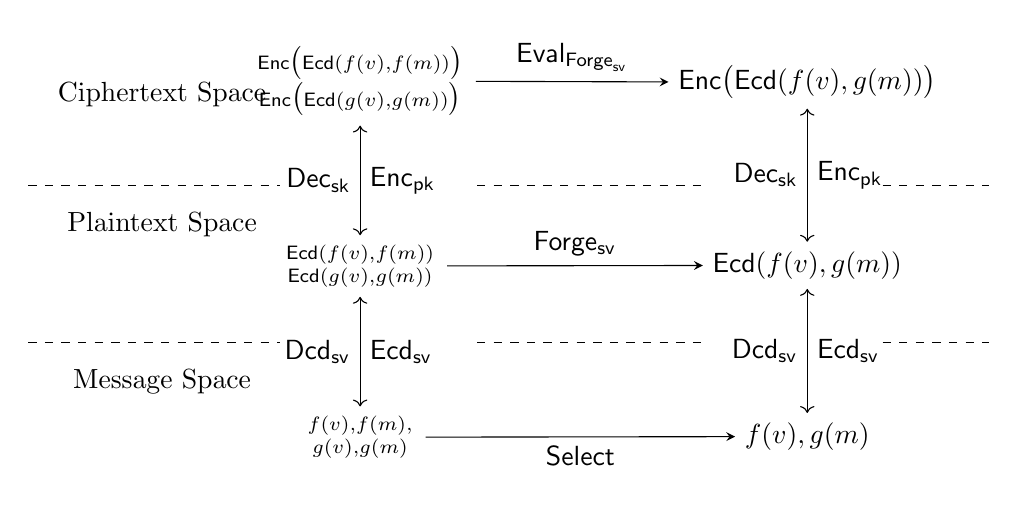
\begin{tikzpicture}
                      \matrix (m) [matrix of math nodes,row sep=4em,column sep=7em,minimum width=2em]
                      {
                        \nobarfrac{\enc\big(\mathsf{Ecd}(f(v), f(m))\big)}{\enc\big(\mathsf{Ecd}(g(v),g(m))\big)} &\enc\big(\mathsf{Ecd}(f(v),g(m))\big)\\
                        \nobarfrac{\mathsf{Ecd}(f(v), f(m))}{\mathsf{Ecd}(g(v),g(m))}&\mathsf{Ecd}(f(v),g(m)) \\
                        \nobarfrac{f(v),f(m),}{g(v),g(m)} & f(v),g(m)\\
                      };
                      \path[]
                        (m-1-1) edge [-stealth] node[above]{\sf Eval$_{\mathsf{Forge}_\mathsf{sv}}$} (m-1-2)
                                edge [<->] node[left] {$\mathsf{Dec_{sk}}$} node[right] {$\mathsf{Enc_{pk}}$} (m-2-1) 
                        (m-1-2) edge [<->] node[left] {$\mathsf{Dec_{sk}}$} node[right] {$\mathsf{Enc_{pk}}$} (m-2-2)
                        (m-2-1) edge [-stealth] node [above] {\sf Forge$_{\mathsf{sv}}$}(m-2-2)
                                edge [<->] node[left] {$\mathsf{Dcd_{sv}}$} node[right] {$\mathsf{Ecd_{sv}}$} (m-3-1)
                        (m-3-1) edge [-stealth] node[below]{\sf Select} (m-3-2)
                        (m-3-2) edge [<->] node[left] {$\mathsf{Dcd_{sv}}$} node[right] {$\mathsf{Ecd_{sv}}$} (m-2-2)
                        ;
                       \draw[dashed] (-7.2, 0.85) -- (-4, 0.85);
                       \draw[dashed] (-1.5, 0.85) -- (1.4, 0.85);
                       \draw[dashed] (3.65, 0.85) -- (5, 0.85);
                
                       \draw[dashed] (-7.2, -1.15) -- (-4, -1.15);
                       \draw[dashed] (-1.5, -1.15) -- (1.4, -1.15);
                       \draw[dashed] (3.65, -1.15) -- (5, -1.15);
                
                       \node at (-5.5,2.0) {Ciphertext Space};
                       \node at (-5.5,0.35) {Plaintext Space};
                       \node at (-5.5,-1.65) {Message Space};
                    \end{tikzpicture}
                    \caption{An Overview of Homomorphic Forgery on Lightweight VHE. $f$ and $g$ denote the requested circuit and a malicious circuit, respectively.} \label{FigForging}
                \end{figure}
                
        For \REP{}, the secret value for Decoding and Encoding is the verification slot $S$. Accordingly, the homomorphic decoding is just masking a ciphertext by multiplying the encryption of $J_S$ and $J_{S^c}$, and the homomorphic encoding is adding ciphertexts masked by $J_S$ and $J_{S^c}$.

        For \PE{}, the decoding involves evaluating at \(Y=\alpha\) and \(Y=0\), while the encoding process interpolates \(\mathbf{m}, \mathbf{v} \in \mathbb{Z}_t^N\) at \(Y=0\) and \(Y=\alpha\) to obtain
        \[
        \mathbf{m} + (\mathbf{v}-\mathbf{m})\alpha^{-1}\cdot Y.
        \]
        According to the earlier perspective that \( {\sf L}^\star := \enc(0) + \enc(1)Y \) can be seen as an encryption of \(0\) and \(\alpha\), interpolating the two ciphertext polynomials \({\sf F}\) and \({\sf G}\) yields
        \begin{align*}   
        &{\sf G}+({\sf F}-{\sf G})\cdot ({\sf L}^\star)^{-1}Y \\
        = &{\sf G}+({\sf F}-{\sf G})\cdot ({\sf L}^\star)^{\phi(t)-1}Y.
        \end{align*}
        This clearly exhibits the structure of the previously discussed cheating circuit.
            
            % prevent the attack on the \REP, there are some patches: 
            % Restricting the operations of HE.
            % But, restricting the operation between ciphertexts by using different keys does not countermeasure this attack (Sec. \ref{subsec: diff keys}). 
            % One of the possibilities is to use SHE (Sec. \ref{subsec:SHE}). 
            % However SHE could only be used in limited situations. 
            % Furthermore, since the security assumption that deep circuits are difficult to implement in SHE is heuristic, we remain uncertain about the security of this approach, especially given that we devised a cheating circuit attack even at bootstrapping depth 1.
    % \subsection{Relation between Confidentiality and Integrity}
    
    % To build a verifiable homomorphic encryption scheme using secret information and precomputed results, the following conditions must be satisfied:
    %     \begin{enumerate}
    %         \item [(A1)] The underlying encoding structure that encodes both the precomputed result and the value to compute is `unforgeable' without the knowledge of certain secret values.
    %         \item [(A2)] Any information regarding the secret values should not be revealed even in the encrypted state through homomorphic computation.
    %     \end{enumerate}
        
    % We observe that although VOPRF in \cite{cryptoeprint:PRF} naively assumes condition (A2), it does not actually satisfy the condition under the given parameters. \REP{} satisfies condition (A1) but fails conditions (A2), since \(\enc(J_S)\) can be revealed. Although the attack on \REP{} described in Theorem~\ref{thm: attack on rep} can be blocked by applying a patch, namely by using multiple secret keys, there exists another forgery attack that does not rely on the interoperability between ciphertexts. Furthermore, \PE{} fails to satisfy condition (A1): Without the knowledge of \(\alpha\), it is possible to encode the messages via \(Y^{\phi(t)}\). Moreover, it is difficult to state that \PE{} satisfies condition (A2), since \(\enc(1,\dots,1)Y\) is an encryption of \(\alpha\) in a certain sense.

    % 만약 Encryption scheme의 confidentality를 이용하여 integrity를 보장하고자 한다면, multiple secret key의 사용을 통하여 [(A1)]과 [(A2)]를 만족시키는 방법이 제시될 수 있다.
        
\section{Conclusion}
In this paper, we proposed the attack against verifiable homomorphic encryption schemes introduced in \cite{VE, cryptoeprint:PRF}.

For the vADDG scheme in \cite{cryptoeprint:PRF}, we introduced a shallow pseudo-random characteristic function to overcome the limitation of bootstrapping depth. When a functional bootstrapping with $k$-bit inputs are allowed, the attack probability is $2^{-\beta/(2^k\ln 2)}$ with computational cost $O(\gamma)$. 
For \REP{} in \cite{VE}, we constructed a circuit that homomorphically calculates the position vector of the common values. This attack has cost $O(n\log t)$ with probability 1. 
Our patching solution using multiple secret keys lowers the success probability into \(O(n^{-1})\), which provides very weak security, possibly against a covert adversary.
For \PE{}, we exploit Euler's theorem to construct a deterministic forgery attack with computational cost $O(\log t)$.

One meaningful approach to decrease the success probability of attacks was to restrict the circuit depth that is homomorphically evaluated. However, as can be seen in the attack on vADDG, a cheating circuit can still be constructed even at shallow depths. Moreover, an adversary can perform forgery despite risking computation failure due to error robustness. Thus, this approach of limiting depth requires further precise analysis.
% \footnote{좀 적어봤느데 잘 안되네. 보완해} 


%which corresponds to the cost of evaluating  $p(y)=y^{\phi(t)}.$

% \dhnote{Also in Appendix~\ref{Appendix A} we suggested another attack against $\PE{}$, in the assumption that $\REQ{}$ acts as $\dec({\mathsf Q}_4(\alpha))=\dec({\mathsf Q}_2(\alpha))$ where ${\mathsf Q}_2(Y)=\REQ{({\mathsf Q}_4(Y))}.$
% This problem is reduced to defining Euclidean division on $\cc R^2_q[Y]$. 
% We note that $\mathsf{Q}_4-\mathsf{Q}_2$ can be modified to a monic relation of $\alpha$ $\mathsf R(X)$. i.e. $\dec(\sf R(\alpha))=0^N$.
% Thereafter the adversary can define the Euclidean division on $\cc R^2_q[Y]$ by this monic ciphertext polynomial and forge the computation result efficiently. The attack probability is 1 and its cost is $O(\log t)$.}

%%%%%%%%%%%%%%%%%%%%%%%%%%%%%%
%       Acknowledgement
%%%%%%%%%%%%%%%%%%%%%%%%%%%%%%

\section*{Acknowledgement}
We would like to thank Damien Stehl{\'e} for his guidance and valuable comments on this research. 

%%%%%%%%%%%%%%%%%%%%%%%%%%%%%%
%       Reference
%%%%%%%%%%%%%%%%%%%%%%%%%%%%%%

\bibliographystyle{alpha}
\bibliography{biblo}

\end{document}
%%%%%%%%%%%%%%%%%%%%%%%%%%%%%%
%       Appendix
%%%%%%%%%%%%%%%%%%%%%%%%%%%%%%
\newpage
\appendix
\section{Analysis on \REQ$^\#$}\label{Appendix A}

    In this appendix, we conduct a cryptanalysis of the scenario where \REQ{} operates under the condition 
        \( 
        \dec(\mathsf{Q}_4(\alpha)) = \dec(\mathsf{Q}_2(\alpha)) 
        \).
    \begin{definition}[\REQ$^\#$]
        \REQ$^\#$ is an oracle which takes a quartic ciphertext polynomial $\mathsf{Q}_4(Y)\in \cc R^2_q[Y]$ as input, and outputs a quadratic polynomial $\mathsf{Q_2}(Y)\in \cc R^2_q[Y]$ satisfying the following:
        $$\mathsf{Dec}(\mathsf{Q}_4(0))=\mathsf{Dec}({\mathsf Q}_2(0)),\;\mathsf{Dec}(\mathsf{Q_4}(\alpha))=\mathsf{Dec}({\mathsf Q_2}(\alpha)).$$
    \end{definition}

    \subsection{Attack on \PE~under $\REQ^\#$} \label{subsec.Attack_PE}
    We now demonstrate that if an adversary gains access to $\REQ^\#$ once, they can execute a deterministic, polynomial-time attack without requiring further access. 
    To successfully pass the verification procedure in \PE, $\mathsf{H}(Y)$, the resulting ciphertext polynomial sent to the client, needs to satisfy the following two properties: 
    \begin{itemize}
        \item $\dec(\mathsf{H}(0)) = \dec(\ct_{\textsf{forged}})$
        \item $\dec(\mathsf{H}(\alpha)) = \dec(\mathsf{F}(\alpha))$
    \end{itemize}
    
    Recall the following circuit $\mathsf H(Y)$ satisfies the desired properties:
        \begin{align}
        \mathsf{H}(Y) := \ct_{\sf forged}+(\mathsf F(Y)-\ct_{\sf forged})Y^{\phi(t)}. \tag{$\ast$} \label{H}
        \end{align}
        
    In this Appendix, we present an alternative method for evaluating \(\mathsf{H}\).
    % However, this forgery is immediately detectable.
    % If the server has executed the circuit correctly, the degree of $Y$ would not grow to $\phi(t)$.
    % 
    \subsubsection{Conventions.}
    For convenience, we establish the following convention:
    Let $\Delta=\left\lfloor\frac{q}{t}\right\rfloor\in \cc R_q$. Then, as an insecure encryption of $1^N=(1,\dots, 1)\in \bb Z_t^N$, the BFV ciphertext $(\Delta,0)\in \cc R^2_q$ is the multiplicative identity in $\cc R^2_q$: For any BFV ciphertext $\ct=(b,a)\in \cc R^2_q$,
    \begin{align*}
        \mathsf{Mult}((b,a),(\Delta,0)) &= \left[\left\lfloor\frac{t}{q}(\Delta b,\Delta a)\right\rceil\right]_q\\
        &=(b,a)\in \cc R^2_q.
    \end{align*}
    This convention justifies expressions such as $(1-\ct)(1+Y)\in \cc R^2_q[Y]$.
    Notably, $Y\in \cc R^2_q[Y]$ means $(\Delta,0)Y\in \cc R^2_q[Y]$.
    Finally, we denote $\mathsf{Mult}(\mathsf{ct}_0, \mathsf{ct}_1)$ as $\mathsf{ct}_0 \cdot \mathsf{ct}_1$.
    
    \subsubsection{Finding Homomorphic Equation on $\alpha$.}
        The degree of $\sf H$ is at least $\phi(t)$, which is exponentially large. Thus if the server has executed the circuit correctly, the degree of $Y$ would not grow to $\phi(t)$. Thus the client can quickly detect that $\mathsf{H}(Y)$ is a forged result.
        Now, we show how to lower the degree of $\mathsf H(Y)$ while keeping $\dec(\mathsf H(\alpha))$ and $\dec(\mathsf H(0))$ to be the same. 
        We show that if the adversary has access to the $\REQ^{\#}$ even once then it can lower the whole degree of $\sf H$. 
        Suppose that $\REQ^{\#}(\mathsf  Q_4(Y))=\mathsf Q_2(Y)$.
        Then, the adversary can learn $\alpha$ in encrypted state: a ciphertext polynomial $\mathsf R(Y):=\mathsf{Q}(Y)-{\mathsf Q_2}(Y)=0$ has $\alpha$ as a zero, in the meaning that 
        $$\dec(\mathsf R(\alpha))=0^N=(0,\dots,0)\in \bb Z^N_t.$$
        For example, in the case of $\bb Z_t$ being a finite field, the adversary can homomorphically implement the Cantor-Zassenhaus algorithm\cite{compuationmathematics} to factorize the homomorphic polynomial equation $\mathsf{R}(Y)$ to get an encryption of $\alpha$.
        This gives advantages to the adversary: By substituting $Y^{\phi(t)} \mapsto \alpha^{\phi(t)-1} Y$ in the definition of $\sf H$ (\ref{H}), the degree of $\mathsf H(Y)$ is lowered while keeping the verification conditions.

        

        
        % Let's define $\ct^{(x)}$ as an encryption of $(x,\dots,x)\in \bb Z_t^N$. 
        % First, consider what happens if the adversary finds $\ct^{(\alpha)}$. 
        % Using the relation $Y-\ct^{(\alpha)}=0$, the adversary can manipulate $\mathsf H(Y)$ while keeping the value of $\mathsf H(0)$ and $\mathsf H(\alpha)$ unchanged. 
        % This can be done simply by transforming it as $Y^{\phi(t)} \mapsto \ct^{(\alpha^{\phi(t)-1})} Y$, so that the evaluations at $Y = 0$ and $Y = \alpha$ have the same decryption. 
        % Therefore the adversary calculates $\mathsf {H}$ by $\mathsf F(Y) + \left(\ct_{\textsf{forged}}-\mathsf F(0)\right)\left(1-\ct^{(\alpha^{\phi(t)-1})}Y\right)$ and passes the verification.
        
        % To find $\ct^{(\alpha)}$, the adversary can use the 오라클.%\REQ{} protocol.
        
        % By the oracle, the adversary can learn $\alpha$ in \emph{encrypted state}. 
        % In \REQ{}, the server reduces a quartic ciphertext polynomial $\mathsf{Q_4}(Y)$ into a quadratic polynomial $\mathsf{Q_2}(Y)$ with the client's help, ensuring that the decryption at $Y = 0$ and $Y = \alpha$ remained the same. 
        % Therefore, the server obtains the following relation on $\alpha$ in encrypted state:
        %     \[
        %         \mathsf{R}(Y):=\mathsf{Q}_4(Y)-\mathsf{Q}_2(Y)=\ct_4Y^4+\ct_3Y^3-\tilde{\ct_2}Y^2-\tilde{\ct_1}Y=\enc(0)
        %     \]
        % Especially, $\mathsf{R}(Y)/Y=\ct_4Y^3+\ct_3Y^2-\tilde{\ct_2}Y-\tilde{\ct_1}$ can be understood as homomorphic cubic equations for each $N$ slots with common zero $Y=\alpha$, although some leading coefficients of cubic polynomials could be zero. 
        % Therefore, the adversary can recover $\ct^{(\alpha)}$ by homomorphically solving these $N$ cubic equations.
        % For example, in the case of $\bb Z_t$ being a finite field, the adversary can homomorphically implement the Cantor-Zassenhaus algorithm\cite{compuationmathematics} to factorize this homomorphic cubic equation.


        \subsubsection{Homomorphic Euclidean Division on $\cc R^2_q[Y]$.}
        Utilizing a homomorphic Cantor-Zassenhaus algorithm is an attractive option, but we suggest a nicer and more efficient way to lower the degree. 
        The substitution $Y^{\phi(t)}$ into $\ct(\alpha^{{\phi(t)-1}})Y$ to preserve the evaluation at $Y=\alpha$ and $Y=0$ can be thought as an homomorphic equation 
        $$Y^{\phi(t)}= \ct{(\alpha^{\phi(t)}-1)}Y \mod{\big(Y^2-\ct{(\alpha)} Y\big)}.$$ 
        In other words, $Y^{\phi(t)}, \ct{(\alpha^{\phi(t)}-1)}Y$ are equal elements in $\cc R^2_q[Y]/(Y^2-\ct{(\alpha)} Y)$ under decryption.
        Instead of considering $\cc R^2_q[Y]/(Y^2-\ct{(\alpha)}Y)$, where $\ct{(\alpha)}$ seems not easily found, we will consider another way:
        Recall that from \REQ$^\#$, we are given another homomorphic relation on $Y=\alpha$ and $Y=0$ as $\mathsf{R}(Y):=\mathsf{Q_4}(Y)-\mathsf{{Q_2}}(Y)$. 
        Therefore, we consider $\cc R^2_q[Y]/(\mathsf{R}(Y))$ and aim to find a ciphertext polynomial $\tilde{\mathsf{H}}(Y)$ with low degree such that $$\mathsf H(Y)=\tilde{\mathsf{H}}(Y) \mod{\mathsf R(Y)}.$$
        But there is another problem. Although $\cc R^2_q[Y]/(\mathsf{R}(Y))$ is well-defined, lowering the degree via modulo $\mathsf{R}(Y)$ is a different matter. 
        For example, the polynomial $3Y^{10} \in \mathbb{Z}[Y] / (2Y)$ cannot be reduced to a degree below 10, because $2Y$ is not a monic polynomial, and therefore the Euclidean division by $2Y$ is not well-defined over $\mathbb{Z}[Y]$.
        A similar problem also arises in $\cc R^2_q[Y]/(\mathsf{R}(Y))$. 
        We will solve this problem by making $\mathsf R(Y)$ as an encryption of a monic polynomial.

        Note that the leading coefficient of $\mathsf{R}(Y)$, say $\mathsf{lc(R)}\in \cc R^2_q$, can be chosen by the adversary as desired before applying $\REQ^{\#}$.
        Therefore, the adversary can proceed as follows: 
        First, let $\mathsf{lc(Q_4)}$ be an encryption of $1^N=(1,\dots,1)$, then apply $\REQ^{\#}$ and get $\mathsf{R}(Y)=\mathsf Q_4(Y)-\mathsf{Q_2}(Y)$.
        Since $\mathsf{lc(R)}$ is an encryption of $1^N$ and the constant term of $\mathsf{R}(Y)$ is an encryption of $0^N$, for simplicity it can modify $\mathsf R(Y)$ to be $\mathsf{R}(Y)=Y^4+\ct_{3}Y^{3}+\cdots+\ct_1Y.$

            \begin{algorithm}
                \caption{Recovering Monic Relation $\mathsf R(Y)$}
                \label{alg:monic relation}
                \begin{algorithmic}[1]
                    \Procedure{$\mathsf{Get\_Monic\_}\mathsf{R}$}{} 
                            \State $\ct_d\gets \ct^{(1)}$ 
                            \State $\mathsf{Q_4(Y)} \gets \sum_{i=0}^4\ct_iY^i$ \Comment{For $i<4$, any valid ciphertext for $\ct_i$ is possible.}
                            \State $\mathsf{Q_2}(Y) \gets \REQ^{\#}(\mathsf{Q_4}(Y))$
                            \State $\mathsf{R_{tmp}}(Y) \gets \mathsf{Q_4}(Y)-\mathsf{Q_2}(Y)$ 
                            \State $\mathsf{R}(Y)\gets \mathsf{R_{tmp}}(Y)-\mathsf{lc(R_{tmp})}Y^4+Y^4-\mathsf{R_{tmp}}(0)$
                            % \Comment{The leading coefficient of $\mathsf{R}$ is substituted to $(\Delta,0)\in \cc R^2_q$, and the constant term is deleted.}
                            \State \Return $\mathsf{R}(Y)$
                    \EndProcedure
                \end{algorithmic}
            \end{algorithm}
            
    Then, the monic relation 
        \[
            \mathsf{R}(Y) = Y^4 +\dots+\ct_1 Y
        \] 
    has zeros at $Y = \alpha$ and $0$ under decryption.
    With this monic polynomial $\mathsf{R}(Y)$, we can define Euclidean division on $\cc R^2_q[Y]$. 
    Although it is similar to the Euclidean division on a polynomial algebra over a ring, we state it here for clarity. 
    Since we are only interested in the remainder polynomial, we do not denote the quotient polynomial. 
    % Here $\mathsf{lc}(\mathsf F(Y))$ denotes the leading coefficient ciphertext of $\mathsf{F}(Y)$.
     
        \begin{algorithm}
            \caption{Homomorphic Euclidean Division on $\cc R^2_q[Y]$ by $\mathsf{R}(Y)$}
            \label{alg:ED}
            \begin{algorithmic}[1]
                \Procedure{$\mathsf{ED}_{\mathsf{R}(Y)}$}{$\mathsf F(Y)$} 
                    \Comment{$\mathsf{F}(Y)\in \cc R^2_q[Y]$, $\deg \mathsf F\geq 4$}
                    \State $\mathsf{Rem}(Y)\gets \mathsf F(Y)$
                    \While {$\deg(\mathsf{Rem})\geq 4$} \label{while begin}
                        \State $\mathsf {Tmp}(Y)\gets \mathsf{lc}(\mathsf {Rem})Y^{\deg(\mathsf{Rem})-4}$ 
                        \State $\mathsf{Rem}(Y)\gets \mathsf{Rem}(Y)-\mathsf{Tmp}(Y)\mathsf{R}(Y)$ \label{Homed. line 6}
                    \EndWhile                   \label{while end}
                    \State \Return $\mathsf{Rem}(Y)$
                \EndProcedure
            \end{algorithmic}
        \end{algorithm}
    
    One might worry if $\mathsf{lc}(\mathsf {Rem})$ is an encryption of the zero vector. 
    However, it does not harm the correctness of the algorithm. 
    Suppose that is the case, then $\mathsf{Tmp}(Y)$ is an encryption of zero polynomial $0\in \bb Z_t^N[Y]$. 
    Thus the decryption of $\mathsf{Rem}(Y)$ is not updated in line \ref{Homed. line 6}, but the degree of $\mathsf{Rem}(Y)$ reduces.

    \begin{lemma}\label{Lemma: Euclidean Division Cost}
        The homomorphic Euclidean division needs at most $3(\deg \mathsf F-3)$ homomorphic multiplications in $\cc R^2_q$.
    \end{lemma}
    \begin{proof}
        $\textsf{ED}_{\mathsf{R}(Y)}(\mathsf{F}(Y))$ calls the \textbf{while} loop in Algorithm \ref{alg:ED} at most $(\deg \mathsf F-3)$ times, where each loop calls $3$ homomorphic multiplication in $\cc R^2_q$ at line \ref{Homed. line 6} in Algorithm \ref{alg:ED}.
        Thus the homomorphic Euclidean division needs $3(\deg \mathsf F-3)$ homomorphic multiplications in $\cc R^2_q$.
    \end{proof}

    \subsubsection{Lowering $\deg\mathsf{H}$ with $\mathsf{R}(Y)$.}
    Now, the adversary is ready to lower the degree of 
    $$\mathsf{H}(Y) := Y^{\phi(t)} \cdot \mathsf{F}(Y) + \left(1 - Y^{\phi(t)}\right) \cdot \ct_{\textsf{forged}}.$$ 
    First, note that directly evaluating \textsf{ED}$_{\mathsf{R}(Y)}(Y^{\phi(t)})$ is costly, since it needs $O(t)$ Euclidean division. 
    However, the adversary can evaluate $Y^{\phi(t)}\in \cc R^2_q[Y]/(\mathsf{R}(Y))$ efficiently by repeatedly squaring $Y$ in $\cc R^2_q[Y]/(\mathsf{R}(Y))$ in $O(\log(\phi(t))$ complexity.
    As a result, the adversary can efficiently calculate $Y^{\phi(t)}=\sum_{i=0}^{3}\ct_iY^i\pmod{\mathsf{R}(Y)}$. 
    Now substituting $Y^{\phi(t)}$ into $\sum_{i=0}^{3}\ct_iY^i$, the following ciphertext polynomial 
        \begin{align}\label{tildeH}
                    \mathsf{\tilde H}(Y) := \left(\sum_{i=0}^{3}\ct_iY^i\right) \cdot \mathsf{F}(Y) + \left(1 - \sum_{i=0}^{3}\ct_iY^i\right) \cdot \ct_{\textsf{forged}}
        \end{align}
    passes the verification. 
    Thus, this attack is possible as long as the adversary is given a nontrivial homomorphic monic relation on $\alpha$. 
    Now we summarize the result.

        \begin{lemma}\label{lemma eucdivisoin}
            Evaluating $Y^{\phi(t)}=\sum_{i=0}^{3}\ct_iY^i\in \cc R^2_q[Y]/(\mathsf{R}(Y))$ costs at most $25\lceil\log t\rceil$ homomorphic multiplication in $\cc R^2_q$. 
        \end{lemma}       
        \begin{proof}
            First, count the number of homomorphic multiplications in $\cc R^2_q$ per each multiplication in $\cc R^2_q[Y]/(\mathsf{R}(Y))$. 
                \begin{itemize}
                    \item Multiplying $\sum_{i=0}^{3}\ct_iY^i$ and $\sum_{i=0}^{3}\ct'_iY^i$ in $\cc R^2_q[Y]$ needs at most $16$ multiplication in $\cc R^2_q$, with output $\mathsf F(Y)$ of degree $\deg\mathsf{F}=6$.
                    \item By Lemma \ref{Lemma: Euclidean Division Cost}, $\mathsf {ED}_{\mathsf{R}(Y)}(\mathsf F(Y))$ needs $9$ homomorphic multiplications in $\cc R^2_q$.
                    \item Adding up together, one multiplication in $\cc R^2_q[Y]/(\mathsf{R}(Y))$ calls at most $25$-multiplication in $\cc R^2_q$.
                \end{itemize}
            To evaluate $Y^{\phi(t)}$ in $\cc R^2_q[Y]/(\mathsf{R}(Y))$, it needs $\lceil\log t\rceil$ homomorphic multiplications in $\cc R^2_q[Y]/(\mathsf{R}(Y))$. 
            Thus in total, it needs at most $25\lceil\log t\rceil$ homomorphic multiplications in $\cc R^2_q$.
        \end{proof}
    
        \begin{theorem}
             If the adversary can access $\REQ^{\#}$, then $\PE$ is broken with probability 1 within $O(\log t)$ homomorphic multiplications in $\cc R^2_q$.
        \end{theorem}
        \begin{proof}
            Immediate from Lemma \ref{lemma eucdivisoin} and the definition of $\tilde{\mathsf{H}}$ in (\ref{tildeH}).
        \end{proof} 
        \begin{corollary}
            \PE{} is not secure in the presence of $\cc A_c^{\cc O_{\REQ^{\#}}}$
        \end{corollary}
        
\end{document}